
% Default to the notebook output style

    


% Inherit from the specified cell style.




    
\documentclass[11pt]{article}

    
    
    \usepackage[T1]{fontenc}
    % Nicer default font (+ math font) than Computer Modern for most use cases
    \usepackage{mathpazo}

    % Basic figure setup, for now with no caption control since it's done
    % automatically by Pandoc (which extracts ![](path) syntax from Markdown).
    \usepackage{graphicx}
    % We will generate all images so they have a width \maxwidth. This means
    % that they will get their normal width if they fit onto the page, but
    % are scaled down if they would overflow the margins.
    \makeatletter
    \def\maxwidth{\ifdim\Gin@nat@width>\linewidth\linewidth
    \else\Gin@nat@width\fi}
    \makeatother
    \let\Oldincludegraphics\includegraphics
    % Set max figure width to be 80% of text width, for now hardcoded.
    \renewcommand{\includegraphics}[1]{\Oldincludegraphics[width=.8\maxwidth]{#1}}
    % Ensure that by default, figures have no caption (until we provide a
    % proper Figure object with a Caption API and a way to capture that
    % in the conversion process - todo).
    \usepackage{caption}
    \DeclareCaptionLabelFormat{nolabel}{}
    \captionsetup{labelformat=nolabel}

    \usepackage{adjustbox} % Used to constrain images to a maximum size 
    \usepackage{xcolor} % Allow colors to be defined
    \usepackage{enumerate} % Needed for markdown enumerations to work
    \usepackage{geometry} % Used to adjust the document margins
    \usepackage{amsmath} % Equations
    \usepackage{amssymb} % Equations
    \usepackage{textcomp} % defines textquotesingle
    % Hack from http://tex.stackexchange.com/a/47451/13684:
    \AtBeginDocument{%
        \def\PYZsq{\textquotesingle}% Upright quotes in Pygmentized code
    }
    \usepackage{upquote} % Upright quotes for verbatim code
    \usepackage{eurosym} % defines \euro
    \usepackage[mathletters]{ucs} % Extended unicode (utf-8) support
    \usepackage[utf8x]{inputenc} % Allow utf-8 characters in the tex document
    \usepackage{fancyvrb} % verbatim replacement that allows latex
    \usepackage{grffile} % extends the file name processing of package graphics 
                         % to support a larger range 
    % The hyperref package gives us a pdf with properly built
    % internal navigation ('pdf bookmarks' for the table of contents,
    % internal cross-reference links, web links for URLs, etc.)
    \usepackage{hyperref}
    \usepackage{longtable} % longtable support required by pandoc >1.10
    \usepackage{booktabs}  % table support for pandoc > 1.12.2
    \usepackage[inline]{enumitem} % IRkernel/repr support (it uses the enumerate* environment)
    \usepackage[normalem]{ulem} % ulem is needed to support strikethroughs (\sout)
                                % normalem makes italics be italics, not underlines
    

    
    
    % Colors for the hyperref package
    \definecolor{urlcolor}{rgb}{0,.145,.698}
    \definecolor{linkcolor}{rgb}{.71,0.21,0.01}
    \definecolor{citecolor}{rgb}{.12,.54,.11}

    % ANSI colors
    \definecolor{ansi-black}{HTML}{3E424D}
    \definecolor{ansi-black-intense}{HTML}{282C36}
    \definecolor{ansi-red}{HTML}{E75C58}
    \definecolor{ansi-red-intense}{HTML}{B22B31}
    \definecolor{ansi-green}{HTML}{00A250}
    \definecolor{ansi-green-intense}{HTML}{007427}
    \definecolor{ansi-yellow}{HTML}{DDB62B}
    \definecolor{ansi-yellow-intense}{HTML}{B27D12}
    \definecolor{ansi-blue}{HTML}{208FFB}
    \definecolor{ansi-blue-intense}{HTML}{0065CA}
    \definecolor{ansi-magenta}{HTML}{D160C4}
    \definecolor{ansi-magenta-intense}{HTML}{A03196}
    \definecolor{ansi-cyan}{HTML}{60C6C8}
    \definecolor{ansi-cyan-intense}{HTML}{258F8F}
    \definecolor{ansi-white}{HTML}{C5C1B4}
    \definecolor{ansi-white-intense}{HTML}{A1A6B2}

    % commands and environments needed by pandoc snippets
    % extracted from the output of `pandoc -s`
    \providecommand{\tightlist}{%
      \setlength{\itemsep}{0pt}\setlength{\parskip}{0pt}}
    \DefineVerbatimEnvironment{Highlighting}{Verbatim}{commandchars=\\\{\}}
    % Add ',fontsize=\small' for more characters per line
    \newenvironment{Shaded}{}{}
    \newcommand{\KeywordTok}[1]{\textcolor[rgb]{0.00,0.44,0.13}{\textbf{{#1}}}}
    \newcommand{\DataTypeTok}[1]{\textcolor[rgb]{0.56,0.13,0.00}{{#1}}}
    \newcommand{\DecValTok}[1]{\textcolor[rgb]{0.25,0.63,0.44}{{#1}}}
    \newcommand{\BaseNTok}[1]{\textcolor[rgb]{0.25,0.63,0.44}{{#1}}}
    \newcommand{\FloatTok}[1]{\textcolor[rgb]{0.25,0.63,0.44}{{#1}}}
    \newcommand{\CharTok}[1]{\textcolor[rgb]{0.25,0.44,0.63}{{#1}}}
    \newcommand{\StringTok}[1]{\textcolor[rgb]{0.25,0.44,0.63}{{#1}}}
    \newcommand{\CommentTok}[1]{\textcolor[rgb]{0.38,0.63,0.69}{\textit{{#1}}}}
    \newcommand{\OtherTok}[1]{\textcolor[rgb]{0.00,0.44,0.13}{{#1}}}
    \newcommand{\AlertTok}[1]{\textcolor[rgb]{1.00,0.00,0.00}{\textbf{{#1}}}}
    \newcommand{\FunctionTok}[1]{\textcolor[rgb]{0.02,0.16,0.49}{{#1}}}
    \newcommand{\RegionMarkerTok}[1]{{#1}}
    \newcommand{\ErrorTok}[1]{\textcolor[rgb]{1.00,0.00,0.00}{\textbf{{#1}}}}
    \newcommand{\NormalTok}[1]{{#1}}
    
    % Additional commands for more recent versions of Pandoc
    \newcommand{\ConstantTok}[1]{\textcolor[rgb]{0.53,0.00,0.00}{{#1}}}
    \newcommand{\SpecialCharTok}[1]{\textcolor[rgb]{0.25,0.44,0.63}{{#1}}}
    \newcommand{\VerbatimStringTok}[1]{\textcolor[rgb]{0.25,0.44,0.63}{{#1}}}
    \newcommand{\SpecialStringTok}[1]{\textcolor[rgb]{0.73,0.40,0.53}{{#1}}}
    \newcommand{\ImportTok}[1]{{#1}}
    \newcommand{\DocumentationTok}[1]{\textcolor[rgb]{0.73,0.13,0.13}{\textit{{#1}}}}
    \newcommand{\AnnotationTok}[1]{\textcolor[rgb]{0.38,0.63,0.69}{\textbf{\textit{{#1}}}}}
    \newcommand{\CommentVarTok}[1]{\textcolor[rgb]{0.38,0.63,0.69}{\textbf{\textit{{#1}}}}}
    \newcommand{\VariableTok}[1]{\textcolor[rgb]{0.10,0.09,0.49}{{#1}}}
    \newcommand{\ControlFlowTok}[1]{\textcolor[rgb]{0.00,0.44,0.13}{\textbf{{#1}}}}
    \newcommand{\OperatorTok}[1]{\textcolor[rgb]{0.40,0.40,0.40}{{#1}}}
    \newcommand{\BuiltInTok}[1]{{#1}}
    \newcommand{\ExtensionTok}[1]{{#1}}
    \newcommand{\PreprocessorTok}[1]{\textcolor[rgb]{0.74,0.48,0.00}{{#1}}}
    \newcommand{\AttributeTok}[1]{\textcolor[rgb]{0.49,0.56,0.16}{{#1}}}
    \newcommand{\InformationTok}[1]{\textcolor[rgb]{0.38,0.63,0.69}{\textbf{\textit{{#1}}}}}
    \newcommand{\WarningTok}[1]{\textcolor[rgb]{0.38,0.63,0.69}{\textbf{\textit{{#1}}}}}
    
    
    % Define a nice break command that doesn't care if a line doesn't already
    % exist.
    \def\br{\hspace*{\fill} \\* }
    % Math Jax compatability definitions
    \def\gt{>}
    \def\lt{<}
    % Document parameters
    \title{SICP-Spring2018}
    
    
    

    % Pygments definitions
    
\makeatletter
\def\PY@reset{\let\PY@it=\relax \let\PY@bf=\relax%
    \let\PY@ul=\relax \let\PY@tc=\relax%
    \let\PY@bc=\relax \let\PY@ff=\relax}
\def\PY@tok#1{\csname PY@tok@#1\endcsname}
\def\PY@toks#1+{\ifx\relax#1\empty\else%
    \PY@tok{#1}\expandafter\PY@toks\fi}
\def\PY@do#1{\PY@bc{\PY@tc{\PY@ul{%
    \PY@it{\PY@bf{\PY@ff{#1}}}}}}}
\def\PY#1#2{\PY@reset\PY@toks#1+\relax+\PY@do{#2}}

\expandafter\def\csname PY@tok@w\endcsname{\def\PY@tc##1{\textcolor[rgb]{0.73,0.73,0.73}{##1}}}
\expandafter\def\csname PY@tok@c\endcsname{\let\PY@it=\textit\def\PY@tc##1{\textcolor[rgb]{0.25,0.50,0.50}{##1}}}
\expandafter\def\csname PY@tok@cp\endcsname{\def\PY@tc##1{\textcolor[rgb]{0.74,0.48,0.00}{##1}}}
\expandafter\def\csname PY@tok@k\endcsname{\let\PY@bf=\textbf\def\PY@tc##1{\textcolor[rgb]{0.00,0.50,0.00}{##1}}}
\expandafter\def\csname PY@tok@kp\endcsname{\def\PY@tc##1{\textcolor[rgb]{0.00,0.50,0.00}{##1}}}
\expandafter\def\csname PY@tok@kt\endcsname{\def\PY@tc##1{\textcolor[rgb]{0.69,0.00,0.25}{##1}}}
\expandafter\def\csname PY@tok@o\endcsname{\def\PY@tc##1{\textcolor[rgb]{0.40,0.40,0.40}{##1}}}
\expandafter\def\csname PY@tok@ow\endcsname{\let\PY@bf=\textbf\def\PY@tc##1{\textcolor[rgb]{0.67,0.13,1.00}{##1}}}
\expandafter\def\csname PY@tok@nb\endcsname{\def\PY@tc##1{\textcolor[rgb]{0.00,0.50,0.00}{##1}}}
\expandafter\def\csname PY@tok@nf\endcsname{\def\PY@tc##1{\textcolor[rgb]{0.00,0.00,1.00}{##1}}}
\expandafter\def\csname PY@tok@nc\endcsname{\let\PY@bf=\textbf\def\PY@tc##1{\textcolor[rgb]{0.00,0.00,1.00}{##1}}}
\expandafter\def\csname PY@tok@nn\endcsname{\let\PY@bf=\textbf\def\PY@tc##1{\textcolor[rgb]{0.00,0.00,1.00}{##1}}}
\expandafter\def\csname PY@tok@ne\endcsname{\let\PY@bf=\textbf\def\PY@tc##1{\textcolor[rgb]{0.82,0.25,0.23}{##1}}}
\expandafter\def\csname PY@tok@nv\endcsname{\def\PY@tc##1{\textcolor[rgb]{0.10,0.09,0.49}{##1}}}
\expandafter\def\csname PY@tok@no\endcsname{\def\PY@tc##1{\textcolor[rgb]{0.53,0.00,0.00}{##1}}}
\expandafter\def\csname PY@tok@nl\endcsname{\def\PY@tc##1{\textcolor[rgb]{0.63,0.63,0.00}{##1}}}
\expandafter\def\csname PY@tok@ni\endcsname{\let\PY@bf=\textbf\def\PY@tc##1{\textcolor[rgb]{0.60,0.60,0.60}{##1}}}
\expandafter\def\csname PY@tok@na\endcsname{\def\PY@tc##1{\textcolor[rgb]{0.49,0.56,0.16}{##1}}}
\expandafter\def\csname PY@tok@nt\endcsname{\let\PY@bf=\textbf\def\PY@tc##1{\textcolor[rgb]{0.00,0.50,0.00}{##1}}}
\expandafter\def\csname PY@tok@nd\endcsname{\def\PY@tc##1{\textcolor[rgb]{0.67,0.13,1.00}{##1}}}
\expandafter\def\csname PY@tok@s\endcsname{\def\PY@tc##1{\textcolor[rgb]{0.73,0.13,0.13}{##1}}}
\expandafter\def\csname PY@tok@sd\endcsname{\let\PY@it=\textit\def\PY@tc##1{\textcolor[rgb]{0.73,0.13,0.13}{##1}}}
\expandafter\def\csname PY@tok@si\endcsname{\let\PY@bf=\textbf\def\PY@tc##1{\textcolor[rgb]{0.73,0.40,0.53}{##1}}}
\expandafter\def\csname PY@tok@se\endcsname{\let\PY@bf=\textbf\def\PY@tc##1{\textcolor[rgb]{0.73,0.40,0.13}{##1}}}
\expandafter\def\csname PY@tok@sr\endcsname{\def\PY@tc##1{\textcolor[rgb]{0.73,0.40,0.53}{##1}}}
\expandafter\def\csname PY@tok@ss\endcsname{\def\PY@tc##1{\textcolor[rgb]{0.10,0.09,0.49}{##1}}}
\expandafter\def\csname PY@tok@sx\endcsname{\def\PY@tc##1{\textcolor[rgb]{0.00,0.50,0.00}{##1}}}
\expandafter\def\csname PY@tok@m\endcsname{\def\PY@tc##1{\textcolor[rgb]{0.40,0.40,0.40}{##1}}}
\expandafter\def\csname PY@tok@gh\endcsname{\let\PY@bf=\textbf\def\PY@tc##1{\textcolor[rgb]{0.00,0.00,0.50}{##1}}}
\expandafter\def\csname PY@tok@gu\endcsname{\let\PY@bf=\textbf\def\PY@tc##1{\textcolor[rgb]{0.50,0.00,0.50}{##1}}}
\expandafter\def\csname PY@tok@gd\endcsname{\def\PY@tc##1{\textcolor[rgb]{0.63,0.00,0.00}{##1}}}
\expandafter\def\csname PY@tok@gi\endcsname{\def\PY@tc##1{\textcolor[rgb]{0.00,0.63,0.00}{##1}}}
\expandafter\def\csname PY@tok@gr\endcsname{\def\PY@tc##1{\textcolor[rgb]{1.00,0.00,0.00}{##1}}}
\expandafter\def\csname PY@tok@ge\endcsname{\let\PY@it=\textit}
\expandafter\def\csname PY@tok@gs\endcsname{\let\PY@bf=\textbf}
\expandafter\def\csname PY@tok@gp\endcsname{\let\PY@bf=\textbf\def\PY@tc##1{\textcolor[rgb]{0.00,0.00,0.50}{##1}}}
\expandafter\def\csname PY@tok@go\endcsname{\def\PY@tc##1{\textcolor[rgb]{0.53,0.53,0.53}{##1}}}
\expandafter\def\csname PY@tok@gt\endcsname{\def\PY@tc##1{\textcolor[rgb]{0.00,0.27,0.87}{##1}}}
\expandafter\def\csname PY@tok@err\endcsname{\def\PY@bc##1{\setlength{\fboxsep}{0pt}\fcolorbox[rgb]{1.00,0.00,0.00}{1,1,1}{\strut ##1}}}
\expandafter\def\csname PY@tok@kc\endcsname{\let\PY@bf=\textbf\def\PY@tc##1{\textcolor[rgb]{0.00,0.50,0.00}{##1}}}
\expandafter\def\csname PY@tok@kd\endcsname{\let\PY@bf=\textbf\def\PY@tc##1{\textcolor[rgb]{0.00,0.50,0.00}{##1}}}
\expandafter\def\csname PY@tok@kn\endcsname{\let\PY@bf=\textbf\def\PY@tc##1{\textcolor[rgb]{0.00,0.50,0.00}{##1}}}
\expandafter\def\csname PY@tok@kr\endcsname{\let\PY@bf=\textbf\def\PY@tc##1{\textcolor[rgb]{0.00,0.50,0.00}{##1}}}
\expandafter\def\csname PY@tok@bp\endcsname{\def\PY@tc##1{\textcolor[rgb]{0.00,0.50,0.00}{##1}}}
\expandafter\def\csname PY@tok@fm\endcsname{\def\PY@tc##1{\textcolor[rgb]{0.00,0.00,1.00}{##1}}}
\expandafter\def\csname PY@tok@vc\endcsname{\def\PY@tc##1{\textcolor[rgb]{0.10,0.09,0.49}{##1}}}
\expandafter\def\csname PY@tok@vg\endcsname{\def\PY@tc##1{\textcolor[rgb]{0.10,0.09,0.49}{##1}}}
\expandafter\def\csname PY@tok@vi\endcsname{\def\PY@tc##1{\textcolor[rgb]{0.10,0.09,0.49}{##1}}}
\expandafter\def\csname PY@tok@vm\endcsname{\def\PY@tc##1{\textcolor[rgb]{0.10,0.09,0.49}{##1}}}
\expandafter\def\csname PY@tok@sa\endcsname{\def\PY@tc##1{\textcolor[rgb]{0.73,0.13,0.13}{##1}}}
\expandafter\def\csname PY@tok@sb\endcsname{\def\PY@tc##1{\textcolor[rgb]{0.73,0.13,0.13}{##1}}}
\expandafter\def\csname PY@tok@sc\endcsname{\def\PY@tc##1{\textcolor[rgb]{0.73,0.13,0.13}{##1}}}
\expandafter\def\csname PY@tok@dl\endcsname{\def\PY@tc##1{\textcolor[rgb]{0.73,0.13,0.13}{##1}}}
\expandafter\def\csname PY@tok@s2\endcsname{\def\PY@tc##1{\textcolor[rgb]{0.73,0.13,0.13}{##1}}}
\expandafter\def\csname PY@tok@sh\endcsname{\def\PY@tc##1{\textcolor[rgb]{0.73,0.13,0.13}{##1}}}
\expandafter\def\csname PY@tok@s1\endcsname{\def\PY@tc##1{\textcolor[rgb]{0.73,0.13,0.13}{##1}}}
\expandafter\def\csname PY@tok@mb\endcsname{\def\PY@tc##1{\textcolor[rgb]{0.40,0.40,0.40}{##1}}}
\expandafter\def\csname PY@tok@mf\endcsname{\def\PY@tc##1{\textcolor[rgb]{0.40,0.40,0.40}{##1}}}
\expandafter\def\csname PY@tok@mh\endcsname{\def\PY@tc##1{\textcolor[rgb]{0.40,0.40,0.40}{##1}}}
\expandafter\def\csname PY@tok@mi\endcsname{\def\PY@tc##1{\textcolor[rgb]{0.40,0.40,0.40}{##1}}}
\expandafter\def\csname PY@tok@il\endcsname{\def\PY@tc##1{\textcolor[rgb]{0.40,0.40,0.40}{##1}}}
\expandafter\def\csname PY@tok@mo\endcsname{\def\PY@tc##1{\textcolor[rgb]{0.40,0.40,0.40}{##1}}}
\expandafter\def\csname PY@tok@ch\endcsname{\let\PY@it=\textit\def\PY@tc##1{\textcolor[rgb]{0.25,0.50,0.50}{##1}}}
\expandafter\def\csname PY@tok@cm\endcsname{\let\PY@it=\textit\def\PY@tc##1{\textcolor[rgb]{0.25,0.50,0.50}{##1}}}
\expandafter\def\csname PY@tok@cpf\endcsname{\let\PY@it=\textit\def\PY@tc##1{\textcolor[rgb]{0.25,0.50,0.50}{##1}}}
\expandafter\def\csname PY@tok@c1\endcsname{\let\PY@it=\textit\def\PY@tc##1{\textcolor[rgb]{0.25,0.50,0.50}{##1}}}
\expandafter\def\csname PY@tok@cs\endcsname{\let\PY@it=\textit\def\PY@tc##1{\textcolor[rgb]{0.25,0.50,0.50}{##1}}}

\def\PYZbs{\char`\\}
\def\PYZus{\char`\_}
\def\PYZob{\char`\{}
\def\PYZcb{\char`\}}
\def\PYZca{\char`\^}
\def\PYZam{\char`\&}
\def\PYZlt{\char`\<}
\def\PYZgt{\char`\>}
\def\PYZsh{\char`\#}
\def\PYZpc{\char`\%}
\def\PYZdl{\char`\$}
\def\PYZhy{\char`\-}
\def\PYZsq{\char`\'}
\def\PYZdq{\char`\"}
\def\PYZti{\char`\~}
% for compatibility with earlier versions
\def\PYZat{@}
\def\PYZlb{[}
\def\PYZrb{]}
\makeatother


    % Exact colors from NB
    \definecolor{incolor}{rgb}{0.0, 0.0, 0.5}
    \definecolor{outcolor}{rgb}{0.545, 0.0, 0.0}



    
    % Prevent overflowing lines due to hard-to-break entities
    \sloppy 
    % Setup hyperref package
    \hypersetup{
      breaklinks=true,  % so long urls are correctly broken across lines
      colorlinks=true,
      urlcolor=urlcolor,
      linkcolor=linkcolor,
      citecolor=citecolor,
      }
    % Slightly bigger margins than the latex defaults
    
    \geometry{verbose,tmargin=1in,bmargin=1in,lmargin=1in,rmargin=1in}
    
    

    \begin{document}
    
    
    \maketitle
    
    

    
    \subsection{大佬镇楼}\label{ux5927ux4f6cux9547ux697c}

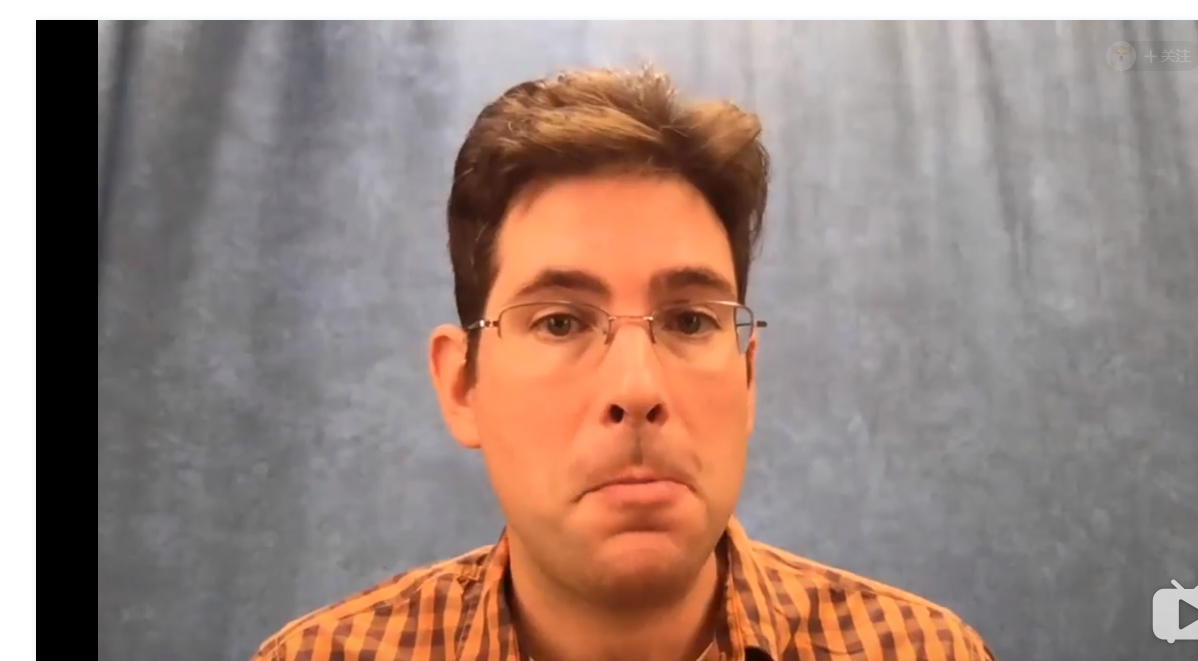
\includegraphics{./image/John.png} \#\#\# 简介 伯克利大学CS61系列第一课
,SICP的Python版本。

    \begin{Verbatim}[commandchars=\\\{\}]
{\color{incolor}In [{\color{incolor} }]:} \PY{c+c1}{\PYZsh{}\PYZsh{}\PYZsh{} 1.3 control}
        \PY{o}{\PYZhy{}} \PY{l+m+mi}{1} \PY{n}{python} \PY{o}{\PYZhy{}}\PY{n}{i} \PY{n}{了解一下} \PY{n}{interactive}
        \PY{o}{\PYZhy{}} \PY{l+m+mi}{2} \PY{n}{pyton} \PY{o}{\PYZhy{}}\PY{n}{m} \PY{n}{了解一下} \PY{o}{\PYZhy{}}\PY{n}{m} \PY{o}{\PYZhy{}}\PY{n}{i}
        \PY{o}{\PYZhy{}} \PY{l+m+mi}{3} \PY{n}{python} \PY{o}{\PYZhy{}}\PY{n}{v} 
        \PY{n}{A} \PY{n}{statement} \PY{o+ow}{is}\PY{p}{:}
        \PY{k+kc}{False} \PY{o+ow}{in} \PY{n}{Python}\PY{err}{:}\PY{k+kc}{False} \PY{l+m+mi}{0} \PY{l+s+s1}{\PYZsq{}}\PY{l+s+s1}{\PYZsq{}} \PY{k+kc}{None}
        \PY{n}{env} \PY{o+ow}{is} \PY{n}{a} \PY{n}{sequence} \PY{n}{of} \PY{n}{frames}
\end{Verbatim}


    \begin{Verbatim}[commandchars=\\\{\}]
{\color{incolor}In [{\color{incolor}3}]:} \PY{k+kn}{from} \PY{n+nn}{operator} \PY{k}{import} \PY{n}{mod}\PY{p}{,}\PY{n}{truediv}\PY{p}{,}\PY{n}{floordiv}
        \PY{n}{mod}\PY{p}{(}\PY{l+m+mi}{2013}\PY{p}{,}\PY{l+m+mi}{5}\PY{p}{)}
\end{Verbatim}


\begin{Verbatim}[commandchars=\\\{\}]
{\color{outcolor}Out[{\color{outcolor}3}]:} 3
\end{Verbatim}
            
    \begin{Verbatim}[commandchars=\\\{\}]
{\color{incolor}In [{\color{incolor}5}]:} \PY{c+c1}{\PYZsh{} Quotient}
\end{Verbatim}


\begin{Verbatim}[commandchars=\\\{\}]
{\color{outcolor}Out[{\color{outcolor}5}]:} 1.0
\end{Verbatim}
            
    \subsubsection{1.4 Higher-order function}\label{higher-order-function}

cs98 addtional Fibobacci seq 与贝壳? 所有递归均可以用非递归方式实现
自上而下 自下而上的备忘录法

function's domain 边界值 function's range 阈值 function's behavior one
job DRY repeat generally \textbf{shared implention:area solution}
函数作为从参数传输进去进行 进行generally 8/(4k-1)(4k-3) = pi Function
are first class:func can be manipulated as a value in program language
Higher Order funtion:A function taht takes a function as an arg value or
ret a func as a ret value

Lambda expression vs def:植物大战僵尸 拉姆达

    \begin{Verbatim}[commandchars=\\\{\}]
{\color{incolor}In [{\color{incolor}9}]:} \PY{k}{assert} \PY{l+m+mi}{3} \PY{o}{\PYZlt{}} \PY{l+m+mi}{2} \PY{p}{,}\PY{l+s+s1}{\PYZsq{}}\PY{l+s+s1}{ Falee}\PY{l+s+s1}{\PYZsq{}}
\end{Verbatim}


    \begin{Verbatim}[commandchars=\\\{\}]

        ---------------------------------------------------------------------------

        AssertionError                            Traceback (most recent call last)

        <ipython-input-9-2baa5041699e> in <module>()
    ----> 1 assert 3 < 2 ,' Falee'
    

        AssertionError:  Falee

    \end{Verbatim}

    \begin{Verbatim}[commandchars=\\\{\}]
{\color{incolor}In [{\color{incolor}11}]:} \PY{k}{def} \PY{n+nf}{make\PYZus{}adder}\PY{p}{(}\PY{n}{n}\PY{p}{)}\PY{p}{:}
             \PY{k}{def} \PY{n+nf}{adder}\PY{p}{(}\PY{n}{k}\PY{p}{)}\PY{p}{:}
                 \PY{k}{return} \PY{n}{k}\PY{o}{+}\PY{n}{n}
             \PY{k}{return} \PY{n}{adder}
\end{Verbatim}


    \begin{Verbatim}[commandchars=\\\{\}]
{\color{incolor}In [{\color{incolor}13}]:} \PY{n}{make\PYZus{}adder}\PY{p}{(}\PY{l+m+mi}{1}\PY{p}{)}\PY{p}{(}\PY{l+m+mi}{10}\PY{p}{)}
\end{Verbatim}


\begin{Verbatim}[commandchars=\\\{\}]
{\color{outcolor}Out[{\color{outcolor}13}]:} 11
\end{Verbatim}
            
    \begin{Verbatim}[commandchars=\\\{\}]
{\color{incolor}In [{\color{incolor}15}]:} \PY{n}{square} \PY{o}{=} \PY{k}{lambda} \PY{n}{x}\PY{p}{:}\PY{n}{x}\PY{o}{*}\PY{n}{x}
\end{Verbatim}


    \subsubsection{1.5 Environment for H\_O
function}\label{environment-for-h_o-function}

类似于Python的装饰器?? 环境类似于Linux fork()函数 frame的概念很重要
关于函数的变量的继承等

    \subsubsection{1.6 Interation}\label{interation}

fibnacci seq kth dif = kth+dif,kth

A call staments is: switch back env fx has a value only one
ret:fork()?? self references

WAV Files

    \begin{Verbatim}[commandchars=\\\{\}]
{\color{incolor}In [{\color{incolor}1}]:} \PY{k}{def} \PY{n+nf}{print\PYZus{}sum}\PY{p}{(}\PY{n}{x}\PY{p}{)}\PY{p}{:}
            \PY{n+nb}{print}\PY{p}{(}\PY{n}{x}\PY{p}{)}
            \PY{k}{def} \PY{n+nf}{next\PYZus{}sum}\PY{p}{(}\PY{n}{y}\PY{p}{)}\PY{p}{:}
                \PY{k}{return} \PY{n}{print\PYZus{}sum}\PY{p}{(}\PY{n}{x}\PY{o}{+}\PY{n}{y}\PY{p}{)}
            \PY{k}{return} \PY{n}{next\PYZus{}sum}
        \PY{n}{print\PYZus{}sum}\PY{p}{(}\PY{l+m+mi}{1}\PY{p}{)}\PY{p}{(}\PY{l+m+mi}{3}\PY{p}{)}\PY{p}{(}\PY{l+m+mi}{5}\PY{p}{)}
\end{Verbatim}


    \begin{Verbatim}[commandchars=\\\{\}]
1
4
9

    \end{Verbatim}

\begin{Verbatim}[commandchars=\\\{\}]
{\color{outcolor}Out[{\color{outcolor}1}]:} <function \_\_main\_\_.print\_sum.<locals>.next\_sum(y)>
\end{Verbatim}
            
    \subsubsection{1.7 recursive function}\label{recursive-function}

call himself directly or not different frames keep diff argument in each
call can be tricky:\textbf{Iteration is a special case of recursion!}
Idea:figure out what state must be cantaintend by the iterative funtion
converting iter to recursion: The state can be passed as arguments
递归结束条件: 自身满足条件结束 Mutual recursion Luhn sum recursion and
iteration

    \begin{Verbatim}[commandchars=\\\{\}]
{\color{incolor}In [{\color{incolor}2}]:} \PY{k}{def} \PY{n+nf}{split}\PY{p}{(}\PY{n}{n}\PY{p}{)}\PY{p}{:}
            \PY{k}{return} \PY{n}{n}\PY{o}{/}\PY{o}{/}\PY{l+m+mi}{10}\PY{p}{,}\PY{n}{n}\PY{o}{\PYZpc{}}\PY{k}{10}
        \PY{k}{def} \PY{n+nf}{sum\PYZus{}digits}\PY{p}{(}\PY{n}{n}\PY{p}{)}\PY{p}{:}
            \PY{k}{if} \PY{n}{n} \PY{o}{\PYZlt{}} \PY{l+m+mi}{10}\PY{p}{:}
                \PY{k}{return} \PY{n}{n}
            \PY{k}{else}\PY{p}{:}
                \PY{n}{all\PYZus{}but\PYZus{}last}\PY{p}{,} \PY{n}{last} \PY{o}{=} \PY{n}{split}\PY{p}{(}\PY{n}{n}\PY{p}{)}
                \PY{k}{return} \PY{n}{sum\PYZus{}digits}\PY{p}{(}\PY{n}{all\PYZus{}but\PYZus{}last}\PY{p}{)} \PY{o}{+} \PY{n}{last}
        \PY{k}{def} \PY{n+nf}{luhn\PYZus{}sum}\PY{p}{(}\PY{p}{)}\PY{p}{:}
            \PY{k}{pass}
\end{Verbatim}


    \begin{Verbatim}[commandchars=\\\{\}]
{\color{incolor}In [{\color{incolor}3}]:} \PY{n}{sum\PYZus{}digits}\PY{p}{(}\PY{l+m+mi}{2013}\PY{p}{)}
\end{Verbatim}


\begin{Verbatim}[commandchars=\\\{\}]
{\color{outcolor}Out[{\color{outcolor}3}]:} 6
\end{Verbatim}
            
    \subsubsection{1.8 Tree recursion}\label{tree-recursion}

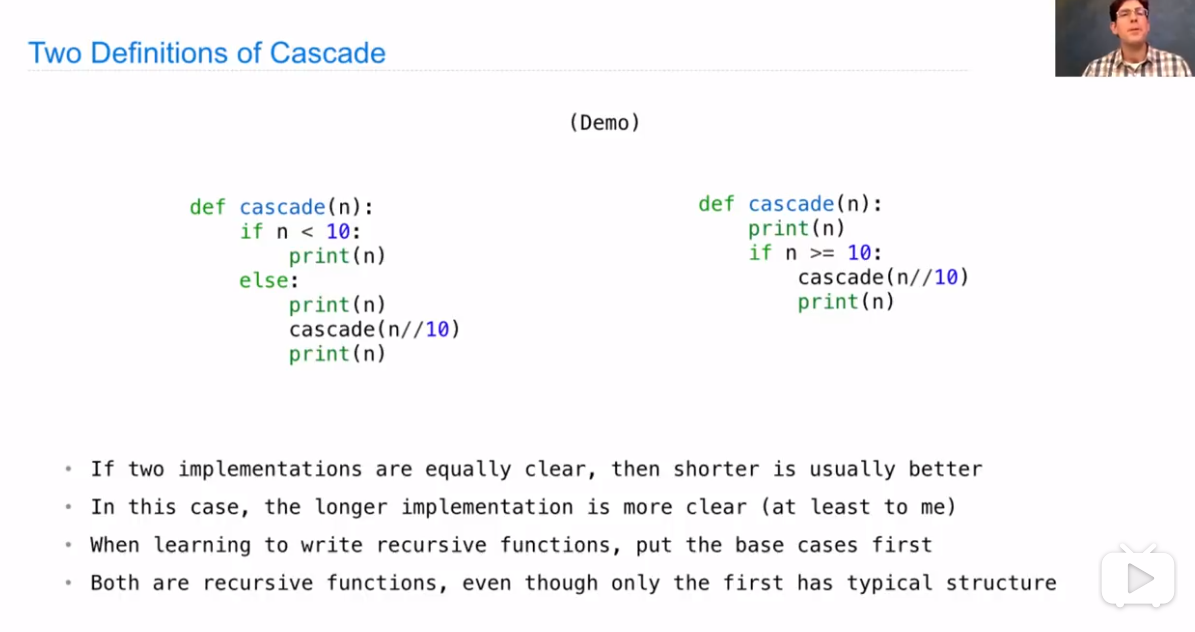
\includegraphics{./image/递归注意事项.png}
递归的重复计算太多很影响时间复杂性!以Fobnacci树为例 到35已经挂了 by
rembering results \#\#\#\# 解决好base case问题 其他交给递归
(感觉很类似于动态规划)

    \begin{Verbatim}[commandchars=\\\{\}]
{\color{incolor}In [{\color{incolor}13}]:} \PY{k+kn}{from} \PY{n+nn}{ucb} \PY{k}{import} \PY{n}{trace}
         \PY{n+nd}{@trace}
         \PY{k}{def} \PY{n+nf}{cascade}\PY{p}{(}\PY{n}{n}\PY{p}{)}\PY{p}{:}
             \PY{k}{if} \PY{n}{n} \PY{o}{\PYZlt{}} \PY{l+m+mi}{10}\PY{p}{:}
                 \PY{k}{pass}
                 \PY{c+c1}{\PYZsh{}print(n)  \PYZsh{}\PYZsh{} base case  return None}
             \PY{k}{else}\PY{p}{:}
                 \PY{c+c1}{\PYZsh{}print(n)}
                 \PY{n}{cascade}\PY{p}{(}\PY{n}{n}\PY{o}{/}\PY{o}{/}\PY{l+m+mi}{10}\PY{p}{)}
                 \PY{c+c1}{\PYZsh{}print(n)}
         \PY{k}{def} \PY{n+nf}{cascade\PYZus{}inverse}\PY{p}{(}\PY{p}{)}\PY{p}{:}
             \PY{k}{pass}
         
         \PY{n+nd}{@trace}
         \PY{k}{def} \PY{n+nf}{fib}\PY{p}{(}\PY{n}{n}\PY{p}{)}\PY{p}{:}
             \PY{k}{if} \PY{n}{n}\PY{o}{\PYZlt{}}\PY{o}{=}\PY{l+m+mi}{1}\PY{p}{:}
                 \PY{k}{return} \PY{n}{n}
             \PY{k}{else}\PY{p}{:}
                 \PY{k}{return} \PY{n}{fib}\PY{p}{(}\PY{n}{n}\PY{o}{\PYZhy{}}\PY{l+m+mi}{1}\PY{p}{)} \PY{o}{+} \PY{n}{fib}\PY{p}{(}\PY{n}{n}\PY{o}{\PYZhy{}}\PY{l+m+mi}{2}\PY{p}{)}
\end{Verbatim}


    \begin{Verbatim}[commandchars=\\\{\}]
{\color{incolor}In [{\color{incolor}15}]:} \PY{c+c1}{\PYZsh{}cascade(12345)}
         \PY{c+c1}{\PYZsh{}fib(10)}
\end{Verbatim}


    \begin{Verbatim}[commandchars=\\\{\}]
{\color{incolor}In [{\color{incolor}19}]:} \PY{c+c1}{\PYZsh{}\PYZsh{} countingh partions}
         \PY{c+c1}{\PYZsh{}\PYZsh{} description : 把一个数分n为几个数的和 最大数不超过m 求多少种分法}
         \PY{k}{def} \PY{n+nf}{count\PYZus{}partion}\PY{p}{(}\PY{n}{n}\PY{p}{,}\PY{n}{m}\PY{p}{)}\PY{p}{:}
             \PY{k}{if} \PY{n}{n} \PY{o}{==} \PY{l+m+mi}{0}\PY{p}{:}
                 \PY{k}{return} \PY{l+m+mi}{1}
             \PY{k}{elif} \PY{n}{n} \PY{o}{\PYZlt{}} \PY{l+m+mi}{0}\PY{p}{:}
                 \PY{k}{return} \PY{l+m+mi}{0}
             \PY{k}{elif} \PY{n}{m} \PY{o}{==} \PY{l+m+mi}{0} \PY{p}{:}
                 \PY{k}{return} \PY{l+m+mi}{0}
             \PY{k}{else}\PY{p}{:}
                 \PY{n}{with\PYZus{}m} \PY{o}{=} \PY{n}{count\PYZus{}partion}\PY{p}{(}\PY{n}{n}\PY{o}{\PYZhy{}}\PY{n}{m}\PY{p}{,}\PY{n}{m}\PY{p}{)}
                 \PY{n}{without\PYZus{}m} \PY{o}{=} \PY{n}{count\PYZus{}partion}\PY{p}{(}\PY{n}{n}\PY{p}{,}\PY{n}{m}\PY{o}{\PYZhy{}}\PY{l+m+mi}{1}\PY{p}{)}
             \PY{k}{return} \PY{n}{with\PYZus{}m} \PY{o}{+} \PY{n}{without\PYZus{}m}
         \PY{n}{count\PYZus{}partion}\PY{p}{(}\PY{l+m+mi}{6}\PY{p}{,}\PY{l+m+mi}{4}\PY{p}{)}
\end{Verbatim}


\begin{Verbatim}[commandchars=\\\{\}]
{\color{outcolor}Out[{\color{outcolor}19}]:} 9
\end{Verbatim}
            
    \subsubsection{1.9 Function Examples}\label{function-examples}

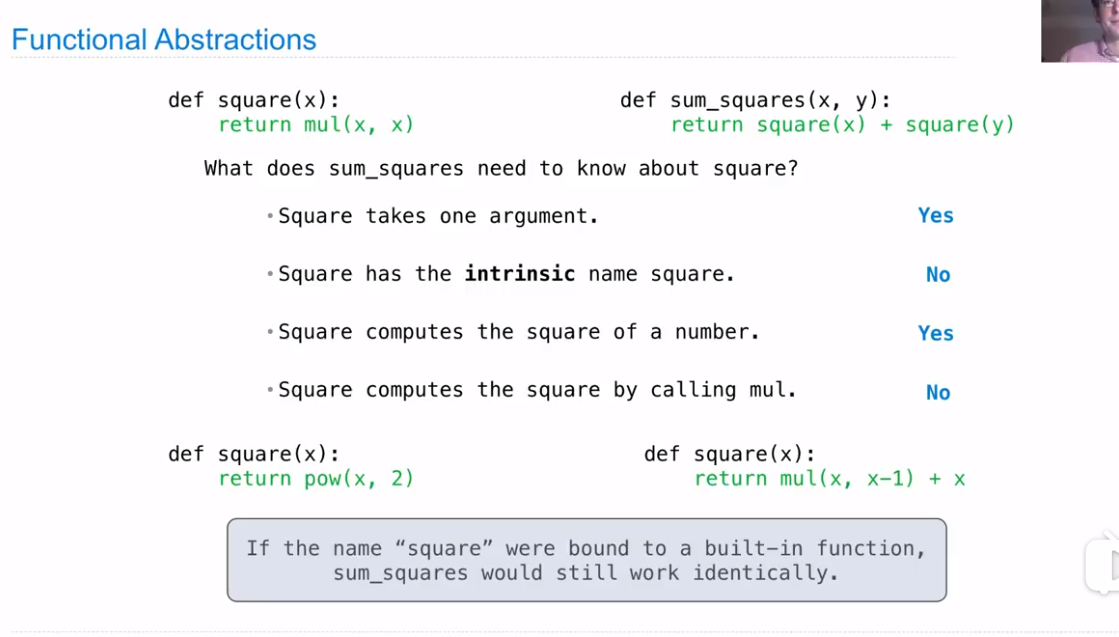
\includegraphics{./image/function_name.png} 函数命名
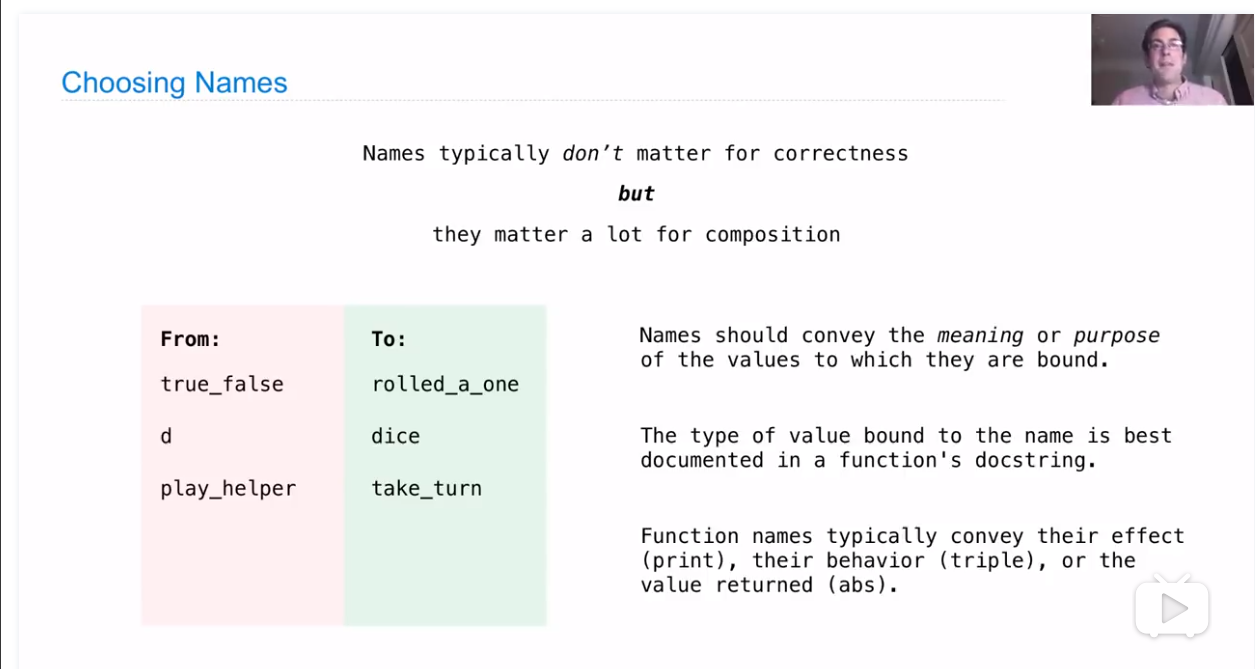
\includegraphics{./image/函数命名.png} 变量命名
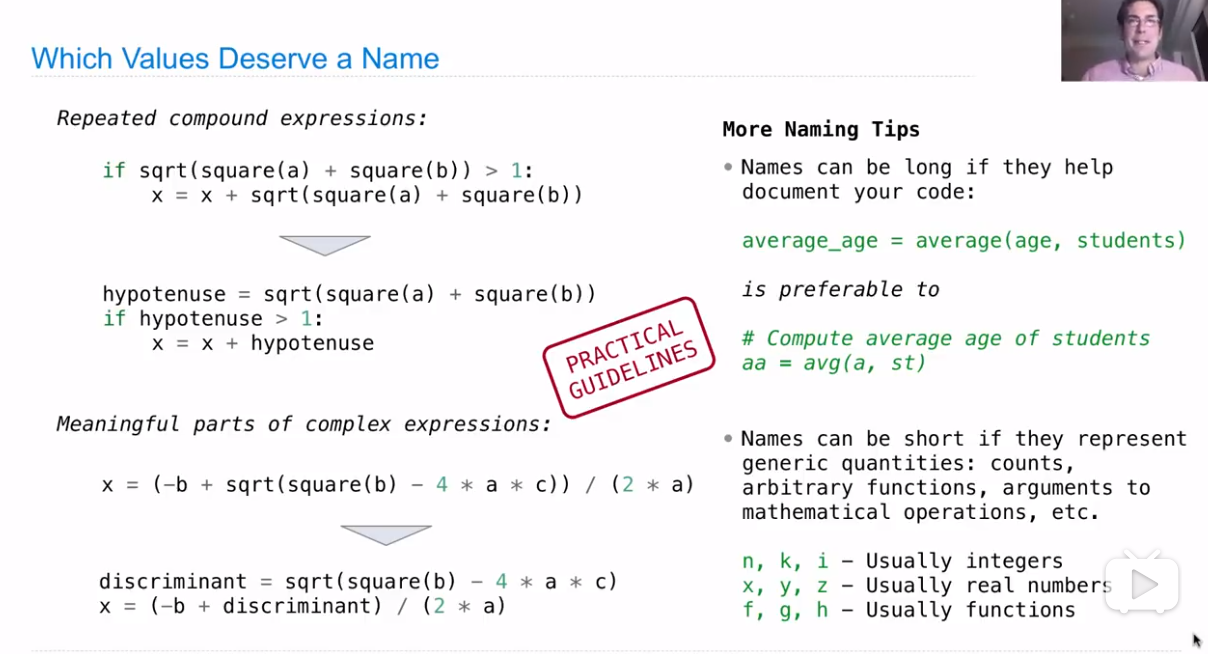
\includegraphics{./image/变量命名.png} - 1 repeated - 2 names can be
long to help depument your code \#\#\#\# Test Driven Development python
-m doctest ex.py \#\#\#\# function currying

\paragraph{Decorators}\label{decorators}

\paragraph{Enclosing scope}\label{enclosing-scope}

\paragraph{}\label{section}

    \begin{Verbatim}[commandchars=\\\{\}]
{\color{incolor}In [{\color{incolor}20}]:} \PY{k}{def} \PY{n+nf}{gcd}\PY{p}{(}\PY{n}{m}\PY{p}{,}\PY{n}{n}\PY{p}{)}\PY{p}{:}
             \PY{l+s+sd}{\PYZsq{}\PYZsq{}\PYZsq{}Return the K largest}
         \PY{l+s+sd}{    k , m, n are all pso}
         \PY{l+s+sd}{    \PYZgt{}\PYZgt{}\PYZgt{} gcd(12,8)}
         \PY{l+s+sd}{    4}
         \PY{l+s+sd}{    \PYZgt{}\PYZgt{}\PYZgt{} gcd(16,12)}
         \PY{l+s+sd}{    4}
         \PY{l+s+sd}{    \PYZsq{}\PYZsq{}\PYZsq{}}
             \PY{k}{if} \PY{n}{m} \PY{o}{==} \PY{n}{n}\PY{p}{:}
                 \PY{k}{return} \PY{n}{m}
             \PY{k}{elif} \PY{n}{m} \PY{o}{\PYZlt{}} \PY{n}{n}\PY{p}{:}
                 \PY{k}{return} \PY{n}{gcd}\PY{p}{(}\PY{n}{n}\PY{p}{,}\PY{n}{m}\PY{p}{)}
             \PY{k}{else}\PY{p}{:}
                 \PY{k}{return} \PY{n}{gcd}\PY{p}{(}\PY{n}{m}\PY{o}{\PYZhy{}}\PY{n}{n}\PY{p}{,}\PY{n}{n}\PY{p}{)}
\end{Verbatim}


    \begin{Verbatim}[commandchars=\\\{\}]
{\color{incolor}In [{\color{incolor}23}]:} \PY{n}{gcd}\PY{p}{(}\PY{l+m+mi}{4}\PY{p}{,}\PY{l+m+mi}{3}\PY{p}{)}
\end{Verbatim}


    \subsubsection{1.10 Data Abstraction}\label{data-abstraction}

数据抽象的意义 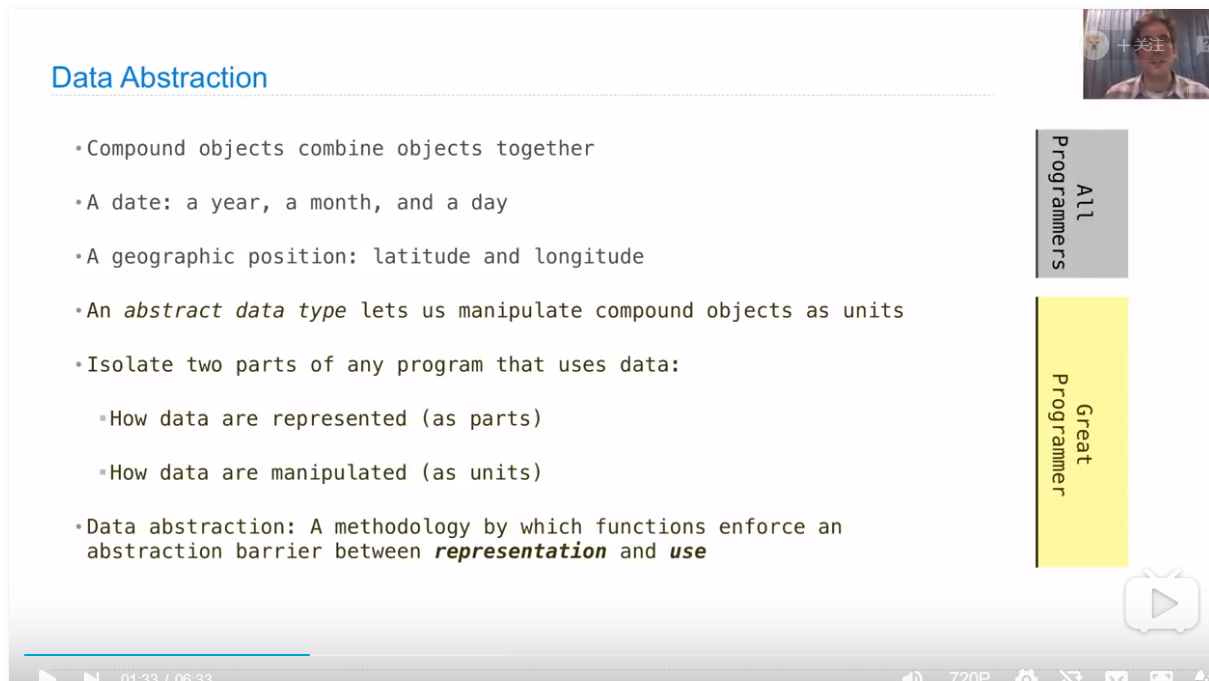
\includegraphics{./image/Data abstraction.png} \#\#\#\#
Pairs \#\#\#\# Abstration Barriers \#\#\#\# Dat a presention

    \begin{Verbatim}[commandchars=\\\{\}]
{\color{incolor}In [{\color{incolor}28}]:} \PY{k+kn}{from} \PY{n+nn}{operator} \PY{k}{import} \PY{n}{getitem}
         \PY{n}{pair} \PY{o}{=} \PY{p}{[}\PY{l+m+mi}{1}\PY{p}{,}\PY{l+m+mi}{2}\PY{p}{]}
         \PY{n}{x}\PY{p}{,} \PY{n}{y} \PY{o}{=} \PY{n}{pair}
         \PY{n}{getitem}\PY{p}{(}\PY{n}{pair}\PY{p}{,}\PY{l+m+mi}{0}\PY{p}{)}
\end{Verbatim}


\begin{Verbatim}[commandchars=\\\{\}]
{\color{outcolor}Out[{\color{outcolor}28}]:} 1
\end{Verbatim}
            
    \subsubsection{1.11 Containers}\label{containers}

\begin{itemize}
\tightlist
\item
  List for in 索引的左闭右开区间{[}-2,2) length: 右减左
  以偏移量作为角标索引
\item
  List Comprehensions 推导
\item
  sring的元素仍为string
\item
  Dict limitation: key不能为可变的的数据 mutable
\end{itemize}

    \begin{Verbatim}[commandchars=\\\{\}]
{\color{incolor}In [{\color{incolor}29}]:} \PY{p}{[}\PY{l+m+mi}{2}\PY{p}{,}\PY{l+m+mi}{7}\PY{p}{]} \PY{o}{+} \PY{p}{[}\PY{l+m+mi}{1}\PY{p}{,}\PY{l+m+mi}{2}\PY{p}{,}\PY{l+m+mi}{3}\PY{p}{]} \PY{o}{*} \PY{l+m+mi}{2}
\end{Verbatim}


\begin{Verbatim}[commandchars=\\\{\}]
{\color{outcolor}Out[{\color{outcolor}29}]:} [2, 7, 1, 2, 3, 1, 2, 3]
\end{Verbatim}
            
    \begin{Verbatim}[commandchars=\\\{\}]
{\color{incolor}In [{\color{incolor}36}]:} \PY{n}{pairs} \PY{o}{=} \PY{p}{[}\PY{p}{[}\PY{l+m+mi}{1}\PY{p}{,}\PY{l+m+mi}{2}\PY{p}{]}\PY{p}{,}\PY{p}{[}\PY{l+m+mi}{3}\PY{p}{,}\PY{l+m+mi}{4}\PY{p}{]}\PY{p}{,}\PY{p}{[}\PY{l+m+mi}{5}\PY{p}{,}\PY{l+m+mi}{6}\PY{p}{]}\PY{p}{,}\PY{p}{[}\PY{l+m+mi}{7}\PY{p}{,}\PY{l+m+mi}{8}\PY{p}{]}\PY{p}{]}
         \PY{k}{for} \PY{n}{x}\PY{p}{,}\PY{n}{y} \PY{o+ow}{in} \PY{n}{pairs}\PY{p}{:}
             \PY{n+nb}{print}\PY{p}{(}\PY{n}{x}\PY{p}{,}\PY{n}{y}\PY{p}{)}
         \PY{n+nb}{range}\PY{p}{(}\PY{o}{\PYZhy{}}\PY{l+m+mi}{2}\PY{p}{,}\PY{l+m+mi}{2}\PY{p}{)}
         \PY{n}{y} \PY{o}{=} \PY{p}{[}\PY{l+m+mi}{1}\PY{p}{,}\PY{l+m+mi}{2}\PY{p}{,}\PY{l+m+mi}{3}\PY{p}{,}\PY{l+m+mi}{4}\PY{p}{,}\PY{l+m+mi}{5}\PY{p}{]}
         \PY{p}{[}\PY{n}{x} \PY{k}{for} \PY{n}{x} \PY{o+ow}{in} \PY{n}{y} \PY{k}{if} \PY{n}{x}\PY{o}{\PYZpc{}}\PY{k}{2} == 0]
\end{Verbatim}


    \begin{Verbatim}[commandchars=\\\{\}]
1 2
3 4
5 6
7 8

    \end{Verbatim}

\begin{Verbatim}[commandchars=\\\{\}]
{\color{outcolor}Out[{\color{outcolor}36}]:} [2, 4]
\end{Verbatim}
            
    \begin{Verbatim}[commandchars=\\\{\}]
{\color{incolor}In [{\color{incolor}37}]:} \PY{p}{\PYZob{}}\PY{n}{x}\PY{p}{:}\PY{n}{x}\PY{o}{*}\PY{o}{*}\PY{n}{x} \PY{k}{for} \PY{n}{x} \PY{o+ow}{in} \PY{n+nb}{range}\PY{p}{(}\PY{l+m+mi}{10}\PY{p}{)}\PY{p}{\PYZcb{}}
\end{Verbatim}


\begin{Verbatim}[commandchars=\\\{\}]
{\color{outcolor}Out[{\color{outcolor}37}]:} \{0: 1,
          1: 1,
          2: 4,
          3: 27,
          4: 256,
          5: 3125,
          6: 46656,
          7: 823543,
          8: 16777216,
          9: 387420489\}
\end{Verbatim}
            
    \subsubsection{1.12 mutable values}\label{mutable-values}

\paragraph{unicode standard}\label{unicode-standard}

\begin{itemize}
\tightlist
\item
  109000 charters
\item
  93 scripts enumeration of charter properties
\end{itemize}

\paragraph{mutation change}\label{mutation-change}

dict.pop(key) \#\#\#\# tuples are sequence but they are not mutable
sequence tuple 不能被改变 用户保护数据 类似于c const?? \textbf{tuple
不能改变 但是元素可以改变!!}

\paragraph{'is' and '=='}\label{is-and}

\begin{itemize}
\tightlist
\item
  is evaluate to Ture if both a and b evaluates the same object
\item
  == evaluate to True if both a and b evaluates the same value identical
  object are always the same value \#\#\#\# mutable values as default
  arg are dangerous
\end{itemize}

    \begin{Verbatim}[commandchars=\\\{\}]
{\color{incolor}In [{\color{incolor}6}]:} \PY{k+kn}{from} \PY{n+nn}{datetime} \PY{k}{import} \PY{n}{date}
        \PY{n+nb}{print}\PY{p}{(}\PY{l+s+s1}{\PYZsq{}}\PY{l+s+se}{\PYZbs{}a}\PY{l+s+se}{\PYZbs{}a}\PY{l+s+se}{\PYZbs{}a}\PY{l+s+s1}{\PYZsq{}}\PY{p}{)} \PY{c+c1}{\PYZsh{}bell}
        \PY{n}{a} \PY{o}{=} \PY{l+s+s1}{\PYZsq{}}\PY{l+s+s1}{A}\PY{l+s+s1}{\PYZsq{}}
        \PY{n+nb}{print}\PY{p}{(}\PY{n+nb}{ord}\PY{p}{(}\PY{n}{a}\PY{p}{)}\PY{p}{,}\PY{n+nb}{hex}\PY{p}{(}\PY{l+m+mi}{65}\PY{p}{)}\PY{p}{)}
\end{Verbatim}


    \begin{Verbatim}[commandchars=\\\{\}]

65 0x41

    \end{Verbatim}

    \begin{Verbatim}[commandchars=\\\{\}]
{\color{incolor}In [{\color{incolor}10}]:} \PY{k+kn}{from} \PY{n+nn}{unicodedata} \PY{k}{import} \PY{n}{lookup}
         \PY{n}{lookup}\PY{p}{(}\PY{l+s+s1}{\PYZsq{}}\PY{l+s+s1}{BABY}\PY{l+s+s1}{\PYZsq{}}\PY{p}{)}
         \PY{n}{a} \PY{o}{=} \PY{p}{(}\PY{p}{[}\PY{l+m+mi}{1}\PY{p}{,}\PY{l+m+mi}{2}\PY{p}{,}\PY{l+m+mi}{3}\PY{p}{]}\PY{p}{,}\PY{l+m+mi}{4}\PY{p}{,}\PY{l+m+mi}{5}\PY{p}{)}
         
         \PY{n+nb}{print}\PY{p}{(}\PY{n}{a}\PY{p}{)}
\end{Verbatim}


    \begin{Verbatim}[commandchars=\\\{\}]
([1, 2, 3], 4, 5)

    \end{Verbatim}

    \begin{Verbatim}[commandchars=\\\{\}]
{\color{incolor}In [{\color{incolor}14}]:} \PY{n}{a}\PY{p}{[}\PY{l+m+mi}{0}\PY{p}{]}\PY{p}{[}\PY{l+m+mi}{1}\PY{p}{]} \PY{o}{=} \PY{l+m+mi}{6} 
         \PY{n+nb}{print}\PY{p}{(}\PY{n}{a}\PY{p}{)}
\end{Verbatim}


    \begin{Verbatim}[commandchars=\\\{\}]
([1, 6, 3], 4, 5)

    \end{Verbatim}

    \begin{Verbatim}[commandchars=\\\{\}]
{\color{incolor}In [{\color{incolor}19}]:} \PY{k}{def} \PY{n+nf}{f}\PY{p}{(}\PY{n}{s} \PY{o}{=} \PY{p}{[}\PY{p}{]}\PY{p}{)}\PY{p}{:}
             \PY{n}{s}\PY{o}{.}\PY{n}{append}\PY{p}{(}\PY{l+m+mi}{1}\PY{p}{)}
             \PY{k}{return} \PY{n+nb}{len}\PY{p}{(}\PY{n}{s}\PY{p}{)}
         \PY{k}{for} \PY{n}{i} \PY{o+ow}{in}  \PY{n+nb}{range}\PY{p}{(}\PY{l+m+mi}{5}\PY{p}{)}\PY{p}{:}
             \PY{n+nb}{print}\PY{p}{(}\PY{n}{f}\PY{p}{(}\PY{p}{)}\PY{p}{)} \PY{n}{really} \PY{n}{dangerous}
\end{Verbatim}


    \begin{Verbatim}[commandchars=\\\{\}]
1
2
3
4
5

    \end{Verbatim}

    \subsubsection{1.14 mutable functions}\label{mutable-functions}

\paragraph{nonlocal statement}\label{nonlocal-statement}

    \subsubsection{1.15 oriented-object
programming}\label{oriented-object-programming}

invoking methods function and method
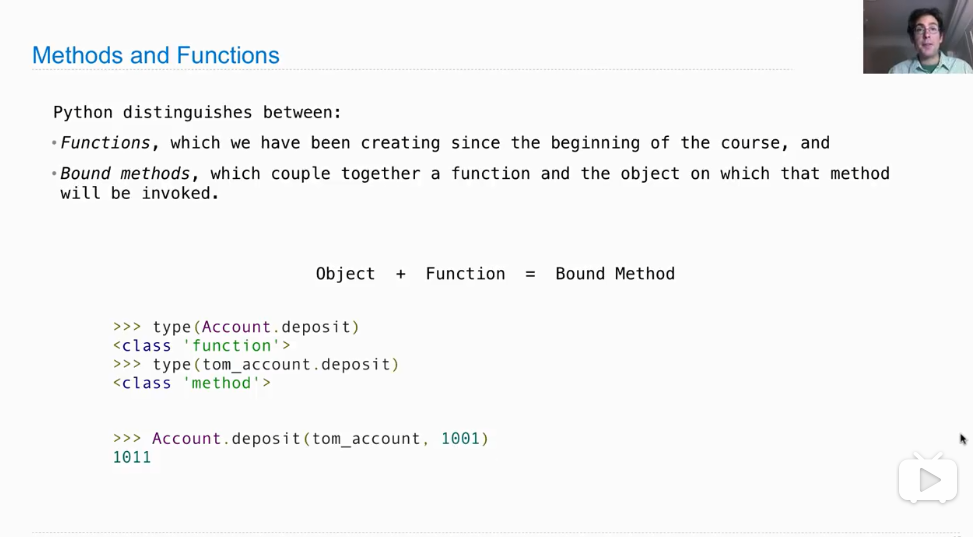
\includegraphics{./image/functionandmethod.png} attribute 很奇怪
为什么可以保存不存在的attr 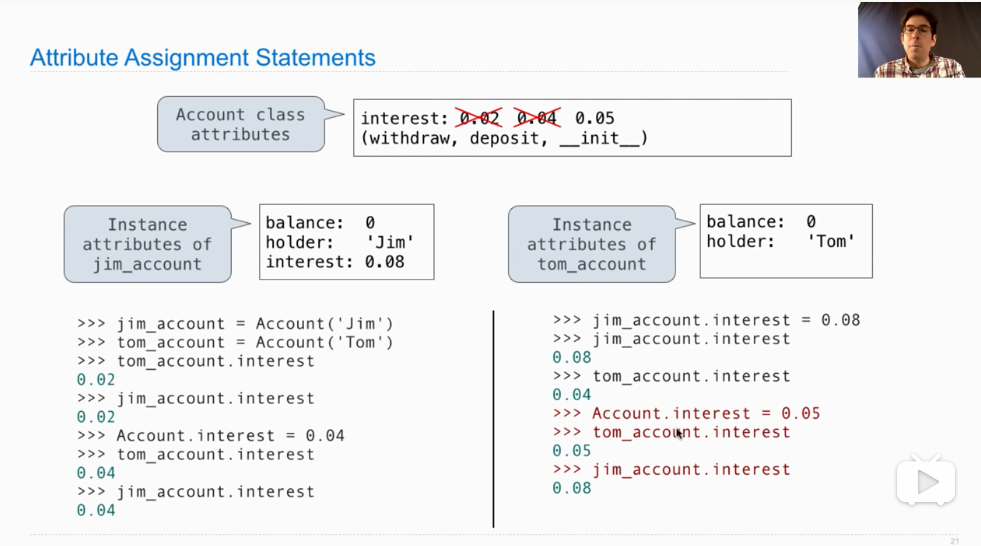
\includegraphics{./image/attribute.png}

    \subsubsection{1.6 inheriate}\label{inheriate}

base class 的attribute 不会拷贝到subclass - attribute lookup
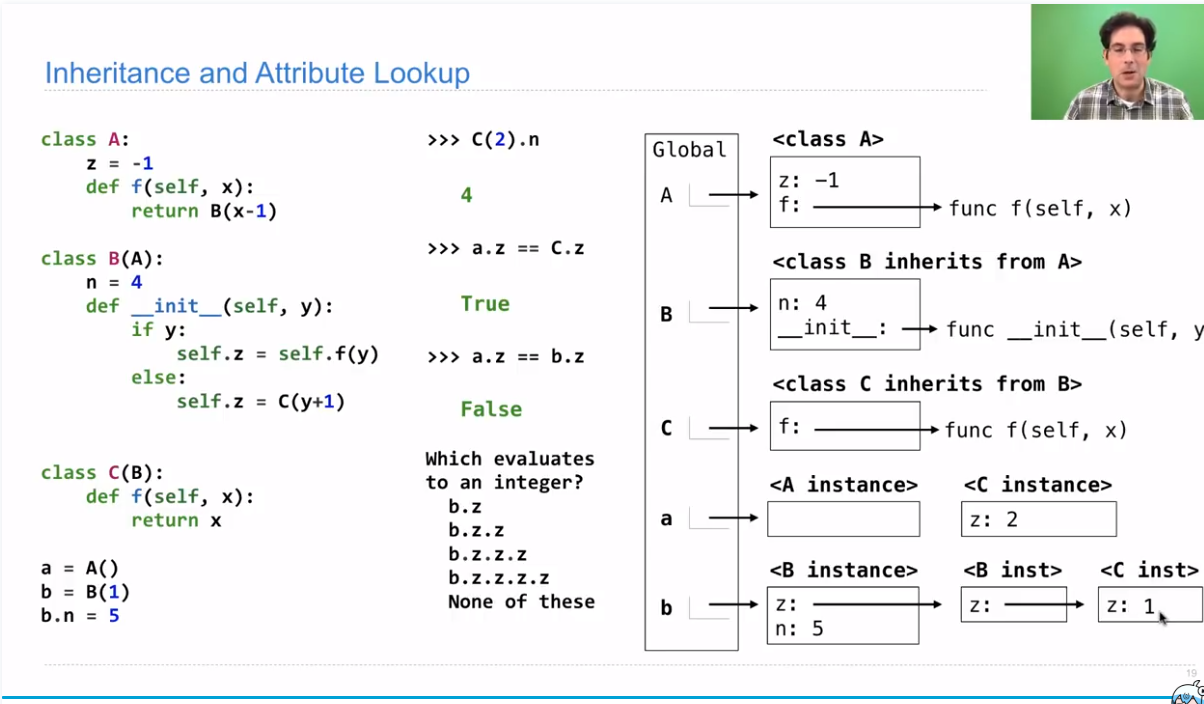
\includegraphics{./image/attribute_lookup.png} - complicated ingeritance

    \subsubsection{1.7 Represention}\label{represention}

\paragraph{str and repr}\label{str-and-repr}

\paragraph{polymorphic functions
多态函数}\label{polymorphic-functions-ux591aux6001ux51fdux6570}

\begin{itemize}
\tightlist
\item
  how implement this behavior \#\#\#\# interface \#\#\#\# special method
  names
\item
  always with two underscores
\item
  \textbf{add} \textbf{str} \textbf{booler} \textbf{float}
\item
  类似于实现多态或者重载
\end{itemize}

    \begin{Verbatim}[commandchars=\\\{\}]
{\color{incolor}In [{\color{incolor}1}]:} \PY{o}{\PYZgt{}\PYZgt{}}\PY{o}{\PYZgt{}} \PY{k+kn}{from} \PY{n+nn}{fractions} \PY{k}{import} \PY{n}{Fraction}
        \PY{o}{\PYZgt{}\PYZgt{}}\PY{o}{\PYZgt{}} \PY{n}{half} \PY{o}{=} \PY{n}{Fraction}\PY{p}{(}\PY{l+m+mi}{1}\PY{p}{,}\PY{l+m+mi}{2}\PY{p}{)}
        \PY{o}{\PYZgt{}\PYZgt{}}\PY{o}{\PYZgt{}} \PY{n+nb}{repr}\PY{p}{(}\PY{n}{half}\PY{p}{)}
        \PY{l+s+s1}{\PYZsq{}}\PY{l+s+s1}{Fraction(1, 2)}\PY{l+s+s1}{\PYZsq{}}
        \PY{o}{\PYZgt{}\PYZgt{}}\PY{o}{\PYZgt{}} \PY{n+nb}{eval}\PY{p}{(}\PY{n+nb}{repr}\PY{p}{(}\PY{n}{half}\PY{p}{)}\PY{p}{)}
        \PY{n}{Fraction}\PY{p}{(}\PY{l+m+mi}{1}\PY{p}{,} \PY{l+m+mi}{2}\PY{p}{)}
\end{Verbatim}


\begin{Verbatim}[commandchars=\\\{\}]
{\color{outcolor}Out[{\color{outcolor}1}]:} Fraction(1, 2)
\end{Verbatim}
            
    \subsubsection{1.18 Growth}\label{growth}

\paragraph{measuring efficency}\label{measuring-efficency}

\paragraph{idea: remeber the result has been
computed}\label{idea-remeber-the-result-has-been-computed}

\begin{itemize}
\tightlist
\item
  装饰器太爽吧 好好看一下
\item
  The consumption of Tine
\item
  求一个数的因数数目。采用平方根的方法快很多。
\item
  Order of Growth
\item
  constant does not affect
\item
  The base of logarithm does not affetx log2等效log10
  O(b\textsuperscript{n) O(n}2) O(n) O(n\^{}0.5) O(logn) O(1)
\item
  Exponentiation
\end{itemize}

b\^{}n 按照n的奇数偶数来分

    \begin{Verbatim}[commandchars=\\\{\}]
{\color{incolor}In [{\color{incolor}21}]:} \PY{c+c1}{\PYZsh{}\PYZsh{}\PYZsh{} 好好理解一下下面代码}
         \PY{k}{def} \PY{n+nf}{fib}\PY{p}{(}\PY{n}{n}\PY{p}{)}\PY{p}{:}
             \PY{k}{if} \PY{n}{n} \PY{o}{\PYZlt{}}\PY{o}{=} \PY{l+m+mi}{1}\PY{p}{:}
                 \PY{k}{return} \PY{n}{n}
             \PY{k}{else}\PY{p}{:}
                 \PY{k}{return} \PY{n}{fib}\PY{p}{(}\PY{n}{n}\PY{o}{\PYZhy{}}\PY{l+m+mi}{1}\PY{p}{)} \PY{o}{+} \PY{n}{fib}\PY{p}{(}\PY{n}{n}\PY{o}{\PYZhy{}}\PY{l+m+mi}{2}\PY{p}{)}
         \PY{k}{def} \PY{n+nf}{count}\PY{p}{(}\PY{n}{f}\PY{p}{)}\PY{p}{:}
             \PY{k}{def} \PY{n+nf}{counted}\PY{p}{(}\PY{n}{n}\PY{p}{)}\PY{p}{:}
                 \PY{n}{counted}\PY{o}{.}\PY{n}{call\PYZus{}count} \PY{o}{+}\PY{o}{=} \PY{l+m+mi}{1}
                 \PY{k}{return} \PY{n}{f}\PY{p}{(}\PY{n}{n}\PY{p}{)}
             \PY{n}{counted}\PY{o}{.}\PY{n}{call\PYZus{}count} \PY{o}{=} \PY{l+m+mi}{0}
             \PY{k}{return} \PY{n}{counted}
         \PY{k}{def} \PY{n+nf}{memo}\PY{p}{(}\PY{n}{f}\PY{p}{)}\PY{p}{:}
             \PY{n}{cache} \PY{o}{=} \PY{p}{\PYZob{}}\PY{p}{\PYZcb{}}
             \PY{k}{def} \PY{n+nf}{memoized}\PY{p}{(}\PY{n}{n}\PY{p}{)}\PY{p}{:}
                 \PY{k}{if} \PY{n}{n} \PY{o+ow}{not} \PY{o+ow}{in} \PY{n}{cache}\PY{p}{:}
                     \PY{n}{cache}\PY{p}{[}\PY{n}{n}\PY{p}{]} \PY{o}{=} \PY{n}{f}\PY{p}{(}\PY{n}{n}\PY{p}{)}
                 \PY{k}{return} \PY{n}{cache}\PY{p}{[}\PY{n}{n}\PY{p}{]}
             \PY{k}{return} \PY{n}{memoized}
         \PY{n+nb}{print}\PY{p}{(}\PY{n}{fib}\PY{p}{(}\PY{l+m+mi}{10}\PY{p}{)}\PY{p}{)}
         \PY{n}{fib} \PY{o}{=} \PY{n}{count}\PY{p}{(}\PY{n}{fib}\PY{p}{)}
         \PY{n+nb}{print}\PY{p}{(}\PY{n}{fib}\PY{p}{(}\PY{l+m+mi}{10}\PY{p}{)}\PY{p}{,}\PY{n}{fib}\PY{o}{.}\PY{n}{call\PYZus{}count}\PY{p}{)}
         \PY{n}{counted\PYZus{}fib} \PY{o}{=} \PY{n}{fib}
         \PY{n}{fib} \PY{o}{=} \PY{n}{memo}\PY{p}{(}\PY{n}{fib}\PY{p}{)}
         \PY{n}{fib} \PY{o}{=} \PY{n}{count}\PY{p}{(}\PY{n}{fib}\PY{p}{)}
         \PY{n+nb}{print}\PY{p}{(}\PY{n}{fib}\PY{p}{(}\PY{l+m+mi}{10}\PY{p}{)}\PY{p}{,}\PY{n}{fib}\PY{o}{.}\PY{n}{call\PYZus{}count}\PY{p}{,}\PY{n}{counted\PYZus{}fib}\PY{o}{.}\PY{n}{call\PYZus{}count}\PY{p}{)}
\end{Verbatim}


    \begin{Verbatim}[commandchars=\\\{\}]
55
55 177
55 19 188

    \end{Verbatim}

    \begin{Verbatim}[commandchars=\\\{\}]
{\color{incolor}In [{\color{incolor}25}]:} \PY{k+kn}{from} \PY{n+nn}{ucb} \PY{k}{import} \PY{n}{trace}
         
         \PY{n+nd}{@trace}
         \PY{k}{def} \PY{n+nf}{exp}\PY{p}{(}\PY{n}{b}\PY{p}{,}\PY{n}{n}\PY{p}{)}\PY{p}{:}
             \PY{k}{if} \PY{n}{n} \PY{o}{==} \PY{l+m+mi}{0}\PY{p}{:}
                 \PY{k}{return} \PY{l+m+mi}{1}
             \PY{k}{else}\PY{p}{:}
                 \PY{k}{return} \PY{n}{b} \PY{o}{*} \PY{n}{exp}\PY{p}{(}\PY{n}{b}\PY{p}{,}\PY{n}{n}\PY{o}{\PYZhy{}}\PY{l+m+mi}{1}\PY{p}{)}
          
         \PY{n+nd}{@trace}
         \PY{k}{def} \PY{n+nf}{fast\PYZus{}exp}\PY{p}{(}\PY{n}{b}\PY{p}{,}\PY{n}{n}\PY{p}{)}\PY{p}{:}
             \PY{k}{if} \PY{n}{n} \PY{o}{==} \PY{l+m+mi}{0}\PY{p}{:}
                 \PY{k}{return} \PY{l+m+mi}{1}
             \PY{k}{elif} \PY{n}{n} \PY{o}{\PYZpc{}} \PY{l+m+mi}{2} \PY{o}{==} \PY{l+m+mi}{0}\PY{p}{:}
                 \PY{k}{return} \PY{n}{square}\PY{p}{(}\PY{n}{fast\PYZus{}exp}\PY{p}{(}\PY{n}{b}\PY{p}{,}\PY{n}{n}\PY{o}{/}\PY{o}{/}\PY{l+m+mi}{2}\PY{p}{)}\PY{p}{)}
             \PY{k}{else}\PY{p}{:}
                 \PY{k}{return} \PY{n}{b} \PY{o}{*} \PY{n}{fast\PYZus{}exp}\PY{p}{(}\PY{n}{b}\PY{p}{,}\PY{n}{n}\PY{o}{\PYZhy{}}\PY{l+m+mi}{1}\PY{p}{)}
             
\end{Verbatim}


    \begin{Verbatim}[commandchars=\\\{\}]
{\color{incolor}In [{\color{incolor}26}]:} \PY{n}{exp}\PY{p}{(}\PY{l+m+mi}{10}\PY{p}{,}\PY{l+m+mi}{5}\PY{p}{)}
\end{Verbatim}


    \begin{Verbatim}[commandchars=\\\{\}]
exp(10, 5):
    exp(10, 4):
        exp(10, 3):
            exp(10, 2):
                exp(10, 1):
                    exp(10, 0):
                    exp(10, 0) -> 1
                exp(10, 1) -> 10
            exp(10, 2) -> 100
        exp(10, 3) -> 1000
    exp(10, 4) -> 10000
exp(10, 5) -> 100000

    \end{Verbatim}

\begin{Verbatim}[commandchars=\\\{\}]
{\color{outcolor}Out[{\color{outcolor}26}]:} 100000
\end{Verbatim}
            
    \subsubsection{1.19 composition}\label{composition}

\begin{itemize}
\tightlist
\item
  Linked list
\item
  property methods
\item
  Tree class
\item
  Tree Mutation
\end{itemize}

    \begin{Verbatim}[commandchars=\\\{\}]
{\color{incolor}In [{\color{incolor}28}]:} \PY{k}{assert} \PY{l+m+mi}{1} \PY{o+ow}{is} \PY{l+m+mi}{1}
\end{Verbatim}


    \subsubsection{1.20 set}\label{set}

s.union s.intersection s.add() \#\#\#\# implementing sets \#\#\#\# sets
as linked liked list - searching an ordered list - set operations def
intersect(set1,set2) - set mutation

    \subsubsection{1.21 Binary Tree}\label{binary-tree}

\paragraph{Binary search :check the middle and eliminate
half}\label{binary-search-check-the-middle-and-eliminate-half}

\paragraph{Bnary search Trees:}\label{bnary-search-trees}

\begin{itemize}
\tightlist
\item
  The biggest element in bst :最右
\item
  The second biggest Tree
  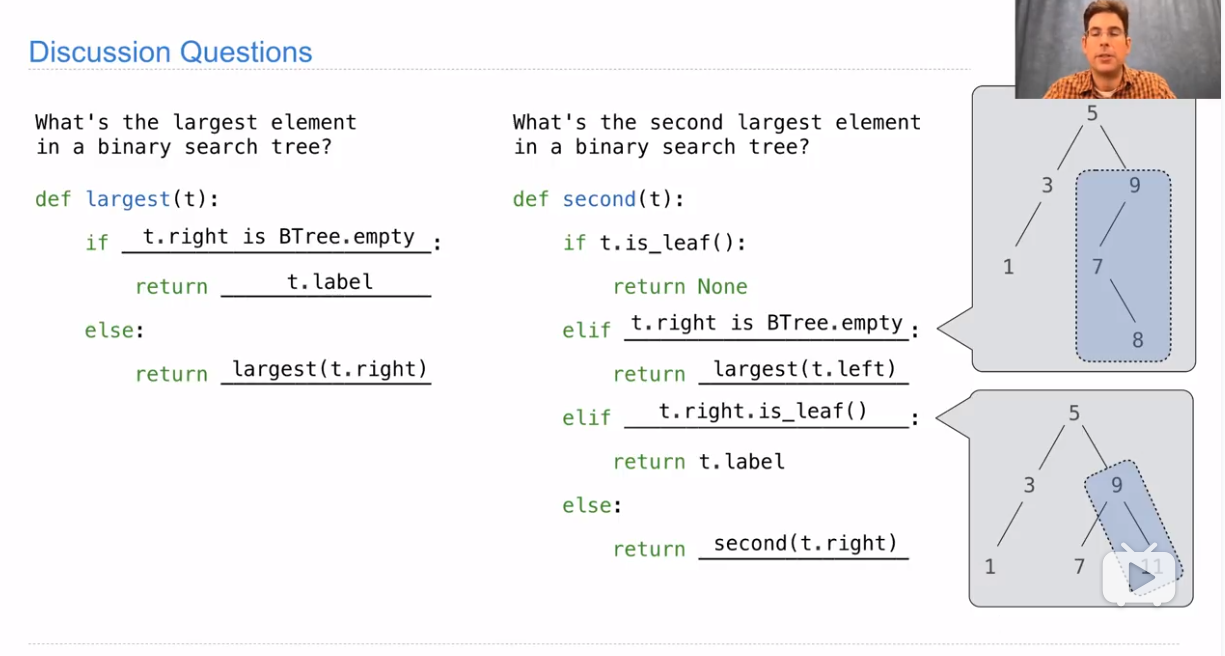
\includegraphics{./image/BiggestElementInTree.png} \#\#\#\# membership
  in BST 每次折半 时间复杂度为logn
\end{itemize}

    \begin{Verbatim}[commandchars=\\\{\}]
{\color{incolor}In [{\color{incolor}29}]:} \PY{k+kn}{from} \PY{n+nn}{random}  \PY{k}{import} \PY{n}{shuffle}
\end{Verbatim}


    \subsubsection{1.22 Data Examples}\label{data-examples}

\begin{itemize}
\tightlist
\item
  List
\item
  append extend addation \%slicing
\item
  list in list 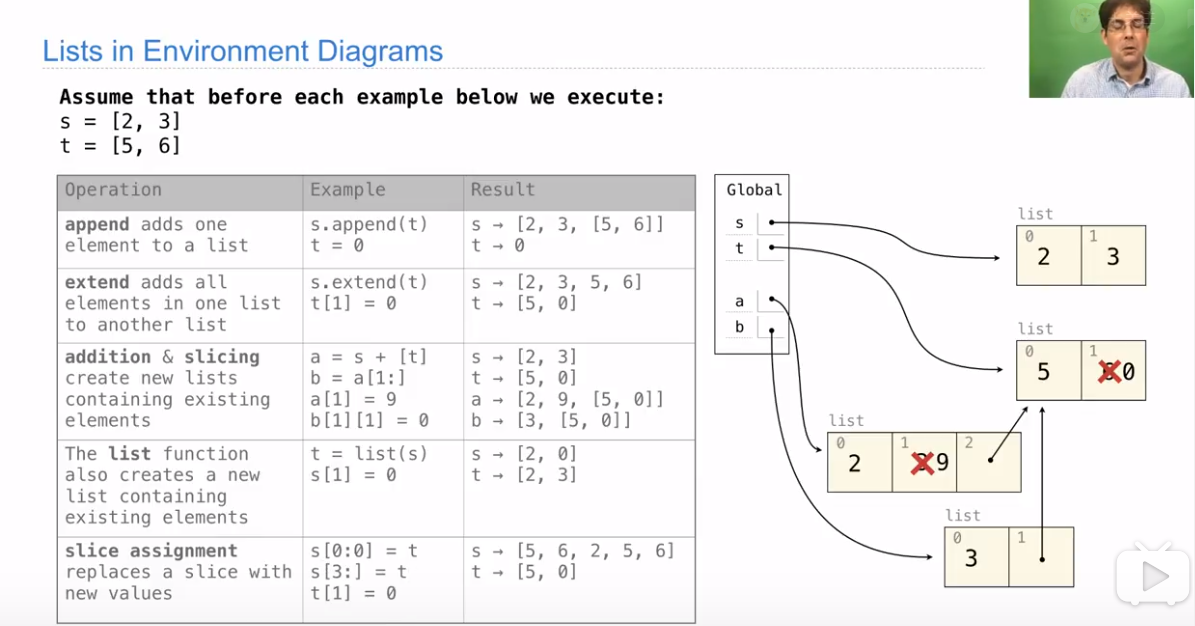
\includegraphics{./image/list_dataex.png} \#\#\#\#
  environment diagram\\
\item
  frame
\item
  parent frame \#\#\#\# objects
\item
  instance 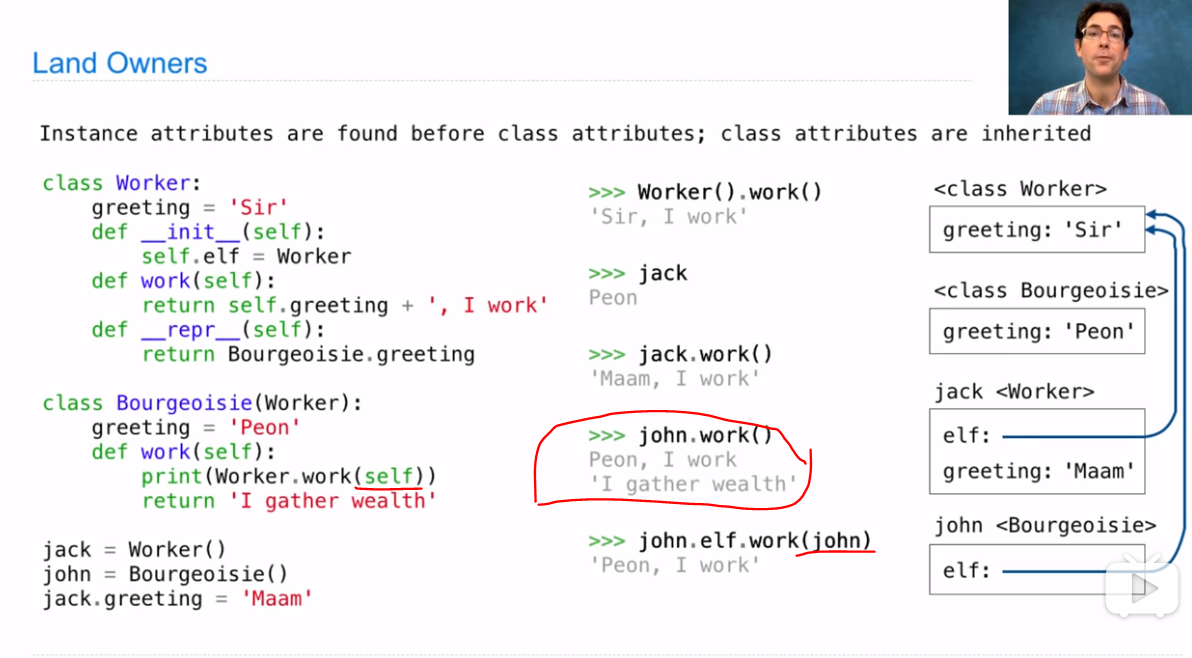
\includegraphics{./image/objects_john.png} \#\#\#\# recursive
  link
\end{itemize}

\paragraph{morse code}\label{morse-code}

    \begin{Verbatim}[commandchars=\\\{\}]
{\color{incolor}In [{\color{incolor}36}]:} \PY{n}{t} \PY{o}{=} \PY{p}{[}\PY{l+m+mi}{1}\PY{p}{,}\PY{l+m+mi}{2}\PY{p}{,}\PY{l+m+mi}{3}\PY{p}{]}
         \PY{n}{t}\PY{p}{[}\PY{l+m+mi}{1}\PY{p}{:}\PY{l+m+mi}{3}\PY{p}{]} \PY{o}{=} \PY{p}{[}\PY{n}{t}\PY{p}{]}
         \PY{n}{t}\PY{o}{.}\PY{n}{extend}\PY{p}{(}\PY{n}{t}\PY{p}{)}
         \PY{n+nb}{print}\PY{p}{(}\PY{n}{t}\PY{p}{,}\PY{n+nb}{len}\PY{p}{(}\PY{n}{t}\PY{p}{[}\PY{l+m+mi}{1}\PY{p}{]}\PY{p}{)}\PY{p}{)}
\end{Verbatim}


    \begin{Verbatim}[commandchars=\\\{\}]
[1, [{\ldots}], 1, [{\ldots}]] 4

    \end{Verbatim}

    \begin{Verbatim}[commandchars=\\\{\}]
{\color{incolor}In [{\color{incolor} }]:} \PY{k}{def} \PY{n+nf}{Worker}\PY{p}{:}
            \PY{n}{g}
\end{Verbatim}


    \subsubsection{1.24}\label{section}

\paragraph{scheme}\label{scheme}

    \subsubsection{1.25 Exceptions}\label{exceptions}

exceptions 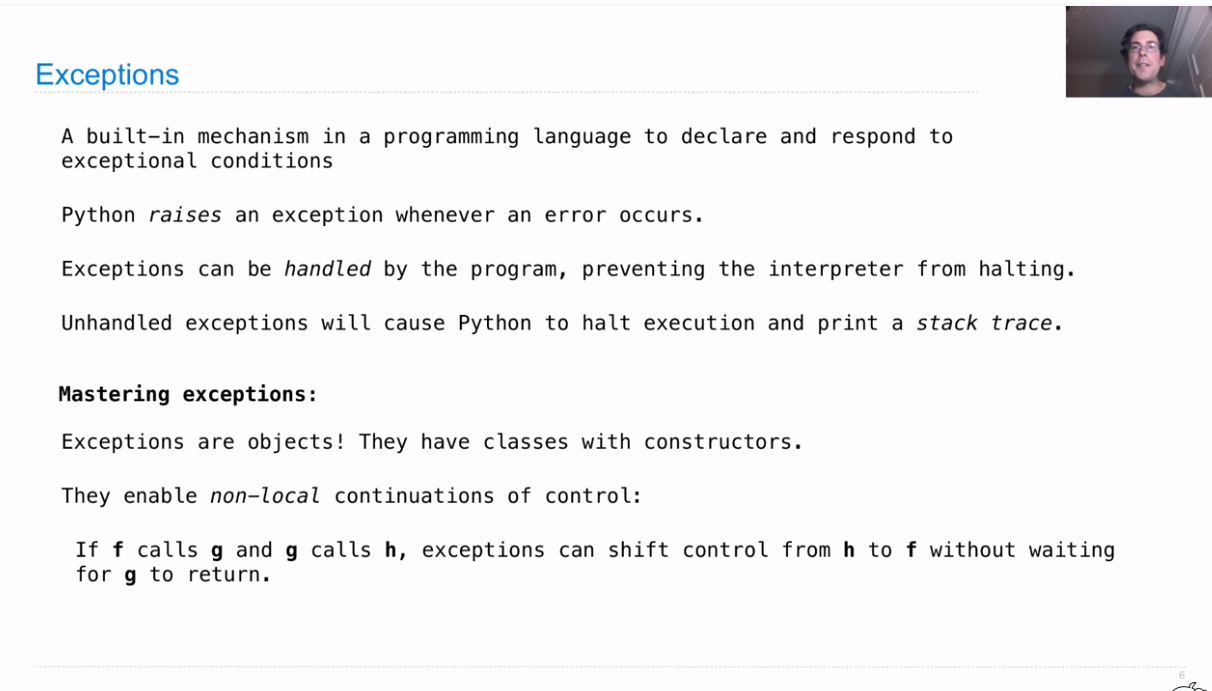
\includegraphics{./image/exceptions.png} \#\#\#\# rasing
exception - assert , assert python -0 ex.py

\paragraph{TypeErr KeyErr NameErr
RuntimeErr(递归过深等)}\label{typeerr-keyerr-nameerr-runtimeerrux9012ux5f52ux8fc7ux6df1ux7b49}

\paragraph{Try statement}\label{try-statement}

\paragraph{WWPD}\label{wwpd}

\paragraph{Reduce:}\label{reduce}

\begin{itemize}
\item
  reduce a sequence to a value \#\#\#\# Sierpinski's triangle
\item
\end{itemize}

    \begin{Verbatim}[commandchars=\\\{\}]
{\color{incolor}In [{\color{incolor}38}]:} \PY{k}{raise} \PY{n+ne}{TypeError}\PY{p}{(}\PY{l+s+s2}{\PYZdq{}}\PY{l+s+s2}{Bad}\PY{l+s+s2}{\PYZdq{}}\PY{p}{)}
         \PY{k}{def} \PY{n+nf}{f}\PY{p}{(}\PY{p}{)}\PY{p}{:}
             \PY{n}{f}\PY{p}{(}\PY{p}{)}
\end{Verbatim}


    \begin{Verbatim}[commandchars=\\\{\}]

        ---------------------------------------------------------------------------

        TypeError                                 Traceback (most recent call last)

        <ipython-input-38-3b635fc5af21> in <module>()
    ----> 1 raise TypeError("Bad")
          2 def f():
          3     f()
    

        TypeError: Bad

    \end{Verbatim}

    \begin{Verbatim}[commandchars=\\\{\}]
{\color{incolor}In [{\color{incolor}41}]:} \PY{k+kn}{from} \PY{n+nn}{operator} \PY{k}{import} \PY{n}{add}
         \PY{n}{reduce}\PY{p}{(}\PY{n}{add}\PY{p}{,}\PY{p}{[}\PY{l+m+mi}{1}\PY{p}{,}\PY{l+m+mi}{2}\PY{p}{,}\PY{l+m+mi}{3}\PY{p}{]}\PY{p}{,}\PY{l+m+mi}{4}\PY{p}{)}
\end{Verbatim}


    \begin{Verbatim}[commandchars=\\\{\}]

        ---------------------------------------------------------------------------

        NameError                                 Traceback (most recent call last)

        <ipython-input-41-6e8e7f9b87a9> in <module>()
          1 from operator import add
    ----> 2 reduce(add,[1,2,3],4)
    

        NameError: name 'reduce' is not defined

    \end{Verbatim}

    \subsubsection{1.26 calculator}\label{calculator}

\subparagraph{Interpreters}\label{interpreters}

\paragraph{parsing}\label{parsing}

    \subsubsection{1.27 Interpreters}\label{interpreters}

Base cases: - scheme evaluation - logical special forms - Quotation

    \subsubsection{1.28 Tail calls}\label{tail-calls}

\paragraph{Dynamic scope}\label{dynamic-scope}

\paragraph{lexical scope}\label{lexical-scope}

\paragraph{tail recursion}\label{tail-recursion}

\paragraph{functional programming}\label{functional-programming}

\paragraph{尾调用 linear recursive can always be re-write as tail
call}\label{ux5c3eux8c03ux7528-linear-recursive-can-always-be-re-write-as-tail-call}

\subsubsection{Map and Reduce Google
论文大作}\label{map-and-reduce-google-ux8bbaux6587ux5927ux4f5c}

\paragraph{An analogy: programs specific
machine}\label{an-analogy-programs-specific-machine}

    \begin{Verbatim}[commandchars=\\\{\}]
{\color{incolor}In [{\color{incolor}45}]:} \PY{n+nb}{list}\PY{p}{(}\PY{n+nb}{map}\PY{p}{(}\PY{n+nb}{abs}\PY{p}{,}\PY{p}{[}\PY{l+m+mi}{1}\PY{p}{,}\PY{l+m+mi}{2}\PY{p}{,}\PY{l+m+mi}{3}\PY{p}{,}\PY{o}{\PYZhy{}}\PY{l+m+mi}{4}\PY{p}{]}\PY{p}{)}\PY{p}{)}
         \PY{n}{reduce}\PY{p}{(}\PY{p}{)}
\end{Verbatim}


\begin{Verbatim}[commandchars=\\\{\}]
{\color{outcolor}Out[{\color{outcolor}45}]:} [1, 2, 3, 4]
\end{Verbatim}
            
    \subsubsection{1.29 Macros}\label{macros}

\subsubsection{1.30 Iterators}\label{iterators}

\paragraph{Data processing}\label{data-processing}

\begin{itemize}
\tightlist
\item
  process squeential data
\item
  sequence interface
\item
  has a finite known lengrh
\item
  allows element selection
\item
  big data processing
\item
  Distributed and parallel computing \#\#\#\# Iterators
\item
  iter return an iterator
\item
  next return the next element in an iterator \#\#\#\# For statements
\item
  when exe for statements ,iter returns an iterator and next provides
  each item
\item
  A StopIteration exception is raised when next is called on empty
  iterator \#\#\#\# bulit-in iterator fnctions 注意啊 iterable
\item
  map() filter(f,iterable) zip() reversed()
  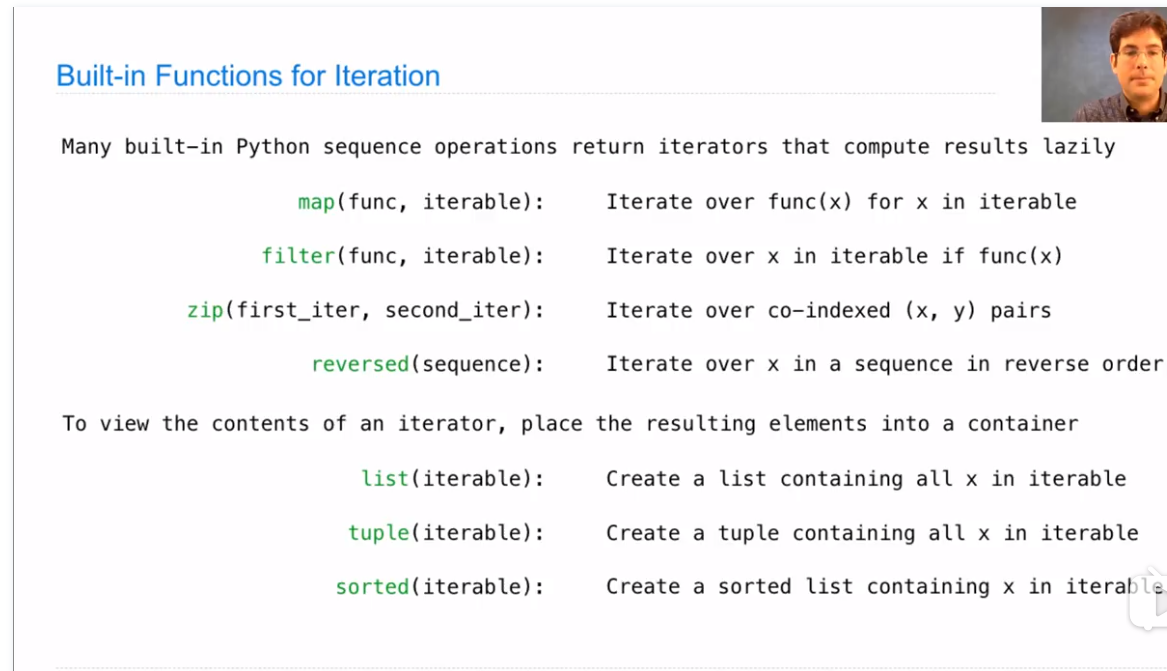
\includegraphics{./image/built-in-iterator.png}
  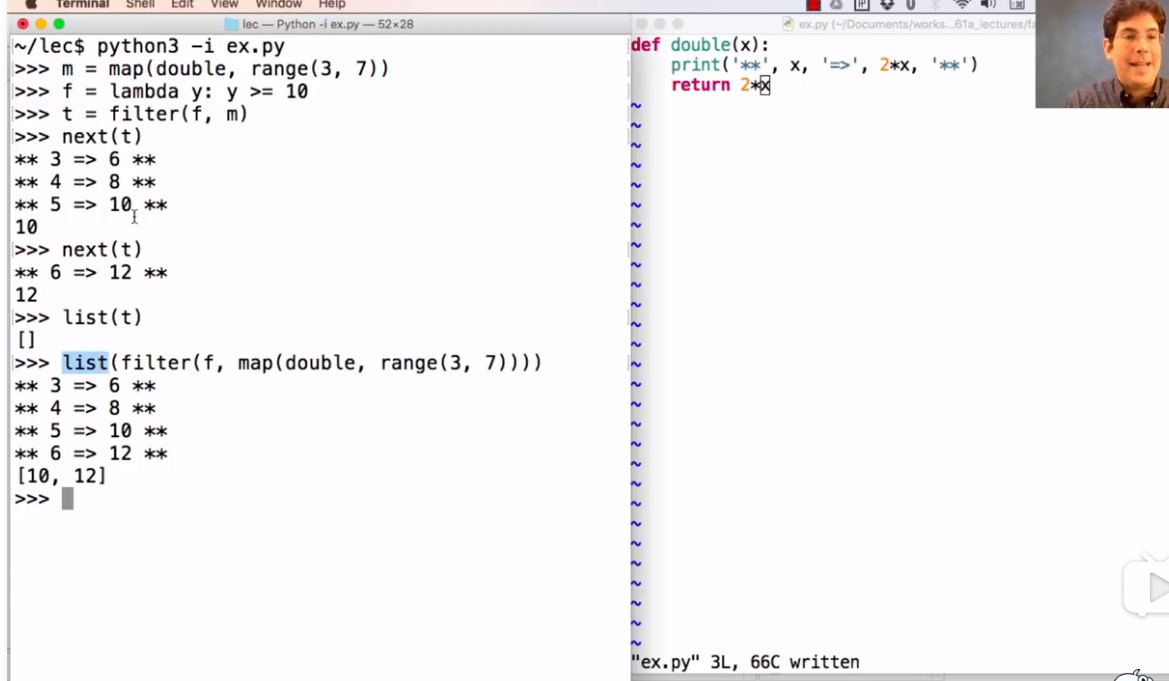
\includegraphics{./image/bulit-in-iter-function.png}
\end{itemize}

\paragraph{Generator and generator
func}\label{generator-and-generator-func}

\begin{itemize}
\tightlist
\item
  yield \#\#\#\# generator and iterator
\item
  genor can Yield from iterator
\item
  yield from 语法
\end{itemize}

    \begin{Verbatim}[commandchars=\\\{\}]
{\color{incolor}In [{\color{incolor}46}]:} \PY{n}{s} \PY{o}{=}\PY{p}{[}\PY{l+m+mi}{11}\PY{p}{,}\PY{l+m+mi}{2}\PY{p}{,}\PY{l+m+mi}{3}\PY{p}{]}
         \PY{n}{t} \PY{o}{=} \PY{n+nb}{iter}\PY{p}{(}\PY{n}{s}\PY{p}{)}
\end{Verbatim}


    \begin{Verbatim}[commandchars=\\\{\}]
{\color{incolor}In [{\color{incolor}49}]:} \PY{n+nb}{next}\PY{p}{(}\PY{n}{t}\PY{p}{)}
         \PY{n+nb}{list}\PY{p}{(}\PY{n}{t}\PY{p}{)}  \PY{c+c1}{\PYZsh{}\PYZsh{} 结束迭代}
\end{Verbatim}


    \begin{Verbatim}[commandchars=\\\{\}]

        ---------------------------------------------------------------------------

        StopIteration                             Traceback (most recent call last)

        <ipython-input-49-1376cbf80061> in <module>()
    ----> 1 next(t)
          2 list(t)
    

        StopIteration: 

    \end{Verbatim}

    \begin{Verbatim}[commandchars=\\\{\}]
{\color{incolor}In [{\color{incolor}51}]:} \PY{n}{d} \PY{o}{=} \PY{p}{\PYZob{}}\PY{l+s+s1}{\PYZsq{}}\PY{l+s+s1}{1}\PY{l+s+s1}{\PYZsq{}}\PY{p}{:}\PY{l+m+mi}{2}\PY{p}{,}\PY{l+s+s1}{\PYZsq{}}\PY{l+s+s1}{2}\PY{l+s+s1}{\PYZsq{}}\PY{p}{:}\PY{l+s+s1}{\PYZsq{}}\PY{l+s+s1}{two}\PY{l+s+s1}{\PYZsq{}}\PY{p}{\PYZcb{}}
         \PY{n}{k} \PY{o}{=} \PY{n+nb}{iter}\PY{p}{(}\PY{n}{d}\PY{p}{)}
\end{Verbatim}


    \begin{Verbatim}[commandchars=\\\{\}]
{\color{incolor}In [{\color{incolor}52}]:} \PY{n+nb}{next}\PY{p}{(}\PY{n}{k}\PY{p}{)}
\end{Verbatim}


\begin{Verbatim}[commandchars=\\\{\}]
{\color{outcolor}Out[{\color{outcolor}52}]:} '1'
\end{Verbatim}
            
    \begin{Verbatim}[commandchars=\\\{\}]
{\color{incolor}In [{\color{incolor}53}]:} \PY{n}{d}\PY{o}{.}\PY{n}{pop}\PY{p}{(}\PY{l+s+s1}{\PYZsq{}}\PY{l+s+s1}{2}\PY{l+s+s1}{\PYZsq{}}\PY{p}{)}
\end{Verbatim}


\begin{Verbatim}[commandchars=\\\{\}]
{\color{outcolor}Out[{\color{outcolor}53}]:} 'two'
\end{Verbatim}
            
    \begin{Verbatim}[commandchars=\\\{\}]
{\color{incolor}In [{\color{incolor}66}]:} \PY{c+c1}{\PYZsh{}\PYZsh{}\PYZsh{} attention}
         \PY{n}{t} \PY{o}{=} \PY{p}{[}\PY{l+m+mi}{1}\PY{p}{,}\PY{l+m+mi}{2}\PY{p}{,}\PY{l+m+mi}{3}\PY{p}{,}\PY{l+m+mi}{2}\PY{p}{,}\PY{l+m+mi}{1}\PY{p}{]}
         \PY{n+nb}{print}\PY{p}{(}\PY{n}{t} \PY{o}{==} \PY{n+nb}{reversed}\PY{p}{(}\PY{n}{t}\PY{p}{)}\PY{p}{,}\PY{n}{t} \PY{o}{==} \PY{n+nb}{list}\PY{p}{(}\PY{n+nb}{reversed}\PY{p}{(}\PY{n}{t}\PY{p}{)}\PY{p}{)}\PY{p}{)}
         
         \PY{n}{d} \PY{o}{=} \PY{p}{\PYZob{}}\PY{l+s+s1}{\PYZsq{}}\PY{l+s+s1}{1}\PY{l+s+s1}{\PYZsq{}}\PY{p}{:}\PY{l+s+s1}{\PYZsq{}}\PY{l+s+s1}{one}\PY{l+s+s1}{\PYZsq{}}\PY{p}{,}\PY{l+s+s1}{\PYZsq{}}\PY{l+s+s1}{2}\PY{l+s+s1}{\PYZsq{}}\PY{p}{:}\PY{l+s+s1}{\PYZsq{}}\PY{l+s+s1}{two}\PY{l+s+s1}{\PYZsq{}}\PY{p}{\PYZcb{}}
         \PY{n}{items} \PY{o}{=} \PY{n+nb}{zip}\PY{p}{(}\PY{n}{d}\PY{o}{.}\PY{n}{keys}\PY{p}{(}\PY{p}{)}\PY{p}{,}\PY{n}{d}\PY{o}{.}\PY{n}{values}\PY{p}{(}\PY{p}{)}\PY{p}{)}
         \PY{n+nb}{print}\PY{p}{(}\PY{n+nb}{list}\PY{p}{(}\PY{n}{items}\PY{p}{)}\PY{p}{)}
         
         
         \PY{c+c1}{\PYZsh{}\PYZsh{} generator}
         \PY{k}{def} \PY{n+nf}{evens}\PY{p}{(}\PY{n}{start}\PY{p}{,}\PY{n}{end}\PY{p}{)}\PY{p}{:}
             \PY{n}{even} \PY{o}{=} \PY{n}{start} \PY{o}{+} \PY{p}{(}\PY{n}{start} \PY{o}{\PYZpc{}} \PY{l+m+mi}{2}\PY{p}{)}
             \PY{k}{while} \PY{n}{even} \PY{o}{\PYZlt{}} \PY{n}{end}\PY{p}{:}
                 \PY{k}{yield} \PY{n}{even}
                 \PY{n}{even} \PY{o}{+}\PY{o}{=} \PY{l+m+mi}{2}
         \PY{n}{g} \PY{o}{=} \PY{n}{evens}\PY{p}{(}\PY{l+m+mi}{2}\PY{p}{,}\PY{l+m+mi}{10}\PY{p}{)}
         \PY{n+nb}{print}\PY{p}{(}\PY{n+nb}{list}\PY{p}{(}\PY{n}{g}\PY{p}{)}\PY{p}{)}
         
         \PY{k}{def} \PY{n+nf}{cntdown}\PY{p}{(}\PY{n}{k}\PY{p}{)}\PY{p}{:}
             \PY{k}{if} \PY{n}{k} \PY{o}{\PYZgt{}} \PY{l+m+mi}{0}\PY{p}{:}
                 \PY{k}{yield} \PY{n}{k}
                 \PY{k}{yield from} \PY{n}{cntdown}\PY{p}{(}\PY{n}{k}\PY{o}{\PYZhy{}}\PY{l+m+mi}{1}\PY{p}{)}
         \PY{k}{for} \PY{n}{k} \PY{o+ow}{in} \PY{n}{cntdown}\PY{p}{(}\PY{l+m+mi}{3}\PY{p}{)}\PY{p}{:}
             \PY{n+nb}{print}\PY{p}{(}\PY{n}{k}\PY{p}{)}
         \PY{n+nb}{print}\PY{p}{(}\PY{n+nb}{list}\PY{p}{(}\PY{n}{cntdown}\PY{p}{(}\PY{l+m+mi}{10}\PY{p}{)}\PY{p}{)}\PY{p}{)}
\end{Verbatim}


    \begin{Verbatim}[commandchars=\\\{\}]
False True
[('1', 'one'), ('2', 'two')]
[2, 4, 6, 8]
3
2
1
[10, 9, 8, 7, 6, 5, 4, 3, 2, 1]

    \end{Verbatim}

    \subsubsection{1.31 streams}\label{streams}

\paragraph{efficent sequence
operations}\label{efficent-sequence-operations}

\paragraph{all()
函数怎么操作的}\label{all-ux51fdux6570ux600eux4e48ux64cdux4f5cux7684}

    \begin{Verbatim}[commandchars=\\\{\}]
{\color{incolor}In [{\color{incolor}4}]:} \PY{n+nb}{all}\PY{p}{(}\PY{n+nb}{map}\PY{p}{(}\PY{k}{lambda} \PY{n}{y}\PY{p}{:} \PY{l+m+mi}{1} \PY{o}{\PYZpc{}} \PY{n}{y}\PY{p}{,}\PY{n+nb}{range}\PY{p}{(}\PY{l+m+mi}{1}\PY{p}{,}\PY{l+m+mi}{6}\PY{p}{)}\PY{p}{)}\PY{p}{)}
\end{Verbatim}


\begin{Verbatim}[commandchars=\\\{\}]
{\color{outcolor}Out[{\color{outcolor}4}]:} False
\end{Verbatim}
            
    \subsubsection{1.32 declarative
programming}\label{declarative-programming}

\paragraph{DataBase Management system
DBMS}\label{database-management-system-dbms}

declarrative langusge 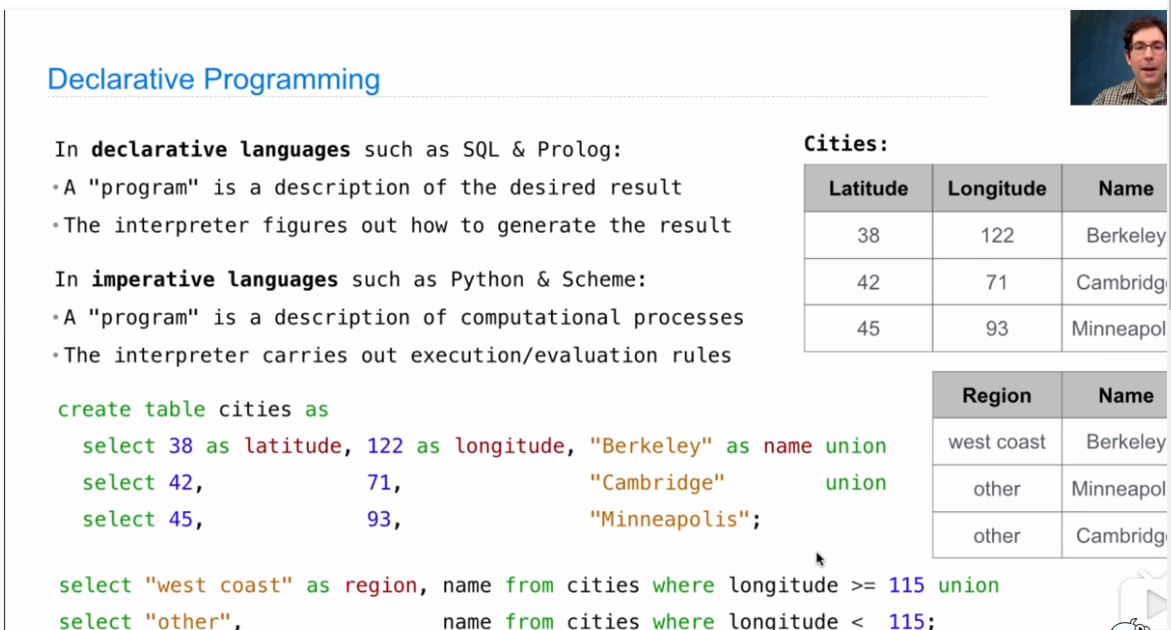
\includegraphics{./image/declarative.png} \#\#\#\#
arithmetic \#\#\# 1.33 Tables pass \#\#\# 1.34 aggregation - SQL专属 -
pass \#\#\#\# 1.35 DataBase - pass \#\#\#\# 1.36 Distributed Data - Unix
- Computer System - Operate System - Networks - DataBase - Dis sys -
Hide complexity but retain flexablity - stdin -\/-\/-\/-\textgreater{}
process -\/-\/-\/-\/-\textgreater{} stdout \textbar{} \textbar{} std err

\begin{itemize}
\tightlist
\item
  sys.stdin sys.std.out
\item
  Big Data
\item
  Apache Spark
\end{itemize}

\begin{figure}
\centering
\includegraphics{./image/DistributedDataset.png}
\caption{}
\end{figure}

\begin{itemize}
\tightlist
\item
  MapReduce
\item
  An important early distributed prossing system developed by google
\end{itemize}

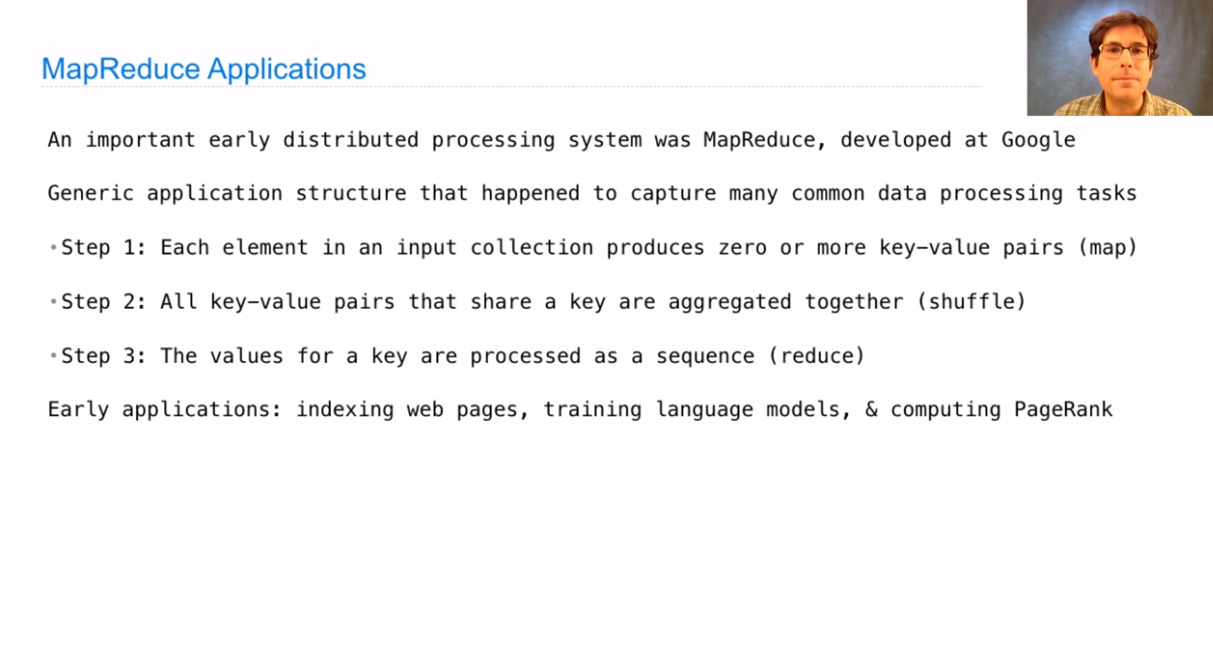
\includegraphics{./image/MapReduceApp.png}
\includegraphics{./image/MpRe-model.png}

    \subsubsection{1.37 Natual language}\label{natual-language}

\paragraph{Ambiguity}\label{ambiguity}

\begin{itemize}
\tightlist
\item
  \textbf{Programs must be written for people to read!}
  -\/-\/-\textgreater{} preface of SICP
\item
  Syntax Trees
\item
  buffalo
\item
  Recursive Tree
\item
  Grammars
\item
  Parsing
\item
  Learning
\end{itemize}

    \emph{end}

    currying rational odd compound civil Comprehensions closure
hierarachical polymorphic arbitrary scheme dialate quotient liberally
useless spatial lextical analysis tokens tail middlemen macros
evaluation Vote cast declarative imperative arithmetic ambiguity
intimidate invoke

柯里 合理的 奇 复合 国内 推导 关闭 hierarachical 多态 随意 方案 dialate
商 宽松 无用 空间的 lextical分析 令牌 尾巴 中间商 宏 评测 投票 陈述
势在必行 算术 歧义 威吓 调用


    % Add a bibliography block to the postdoc
    
    
    
    \end{document}
